

\ifdefined\included
\else
\documentclass[a4paper,11pt,twoside]{StyleThese}
\usepackage{amsmath,amssymb}             % AMS Math
\usepackage[T1]{fontenc}
\usepackage[utf8x]{inputenc}
\usepackage{babel}
\usepackage{datetime}

\usepackage{lmodern}
\usepackage{tabularx}
%\usepackage{tabular}
\usepackage{multirow}

\usepackage{hhline}
\usepackage[left=1.5in,right=1.3in,top=1.1in,bottom=1.1in,includefoot,includehead,headheight=13.6pt]{geometry}
\renewcommand{\baselinestretch}{1.05}

% Table of contents for each chapter

\usepackage[nottoc, notlof, notlot]{tocbibind}
\usepackage{minitoc}
\setcounter{minitocdepth}{2}
\mtcindent=15pt
% Use \minitoc where to put a table of contents

\usepackage{aecompl}

% Glossary / list of abbreviations

\usepackage[intoc]{nomencl}
\iftoggle{ThesisInEnglish}{%
\renewcommand{\nomname}{Glossary}
}{ %
\renewcommand{\nomname}{Liste des Abréviations}
}

\makenomenclature

% My pdf code

\usepackage{ifpdf}

\ifpdf
  \usepackage[pdftex]{graphicx}
  \DeclareGraphicsExtensions{.jpg}
  \usepackage[a4paper,pagebackref,hyperindex=true]{hyperref}
  \usepackage{tikz}
  \usetikzlibrary{arrows,shapes,calc}
\else
  \usepackage{graphicx}
  \DeclareGraphicsExtensions{.ps,.eps}
  \usepackage[a4paper,dvipdfm,pagebackref,hyperindex=true]{hyperref}
\fi

\graphicspath{{.}{images/}}

%% nicer backref links. NOTE: The flag ThesisInEnglish is used to define the
% language in the back references. Read more about it in These.tex

\iftoggle{ThesisInEnglish}{%
\renewcommand*{\backref}[1]{}
\renewcommand*{\backrefalt}[4]{%
\ifcase #1 %
(Not cited.)%
\or
(Cited in page~#2.)%
\else
(Cited in pages~#2.)%
\fi}
\renewcommand*{\backrefsep}{, }
\renewcommand*{\backreftwosep}{ and~}
\renewcommand*{\backreflastsep}{ and~}
}{%
\renewcommand*{\backref}[1]{}
\renewcommand*{\backrefalt}[4]{%
\ifcase #1 %
(Non cité.)%
\or
(Cité en page~#2.)%
\else
(Cité en pages~#2.)%
\fi}
\renewcommand*{\backrefsep}{, }
\renewcommand*{\backreftwosep}{ et~}
\renewcommand*{\backreflastsep}{ et~}
}

% Links in pdf
\usepackage{color}
\definecolor{linkcol}{rgb}{0,0,0.4} 
\definecolor{citecol}{rgb}{0.5,0,0} 
\definecolor{linkcol}{rgb}{0,0,0} 
\definecolor{citecol}{rgb}{0,0,0}
% Change this to change the informations included in the pdf file

\hypersetup
{
bookmarksopen=true,
pdftitle="Évaluation de la sécurité des équipements grand public connectés à Internet",
pdfauthor="Yann BACHY", %auteur du document
pdfsubject="Thèse", %sujet du document
%pdftoolbar=false, %barre d'outils non visible
pdfmenubar=true, %barre de menu visible
pdfhighlight=/O, %effet d'un clic sur un lien hypertexte
colorlinks=true, %couleurs sur les liens hypertextes
pdfpagemode=None, %aucun mode de page
pdfpagelayout=SinglePage, %ouverture en simple page
pdffitwindow=true, %pages ouvertes entierement dans toute la fenetre
linkcolor=linkcol, %couleur des liens hypertextes internes
citecolor=citecol, %couleur des liens pour les citations
urlcolor=linkcol %couleur des liens pour les url
}

% definitions.
% -------------------

\setcounter{secnumdepth}{3}
\setcounter{tocdepth}{2}

% Some useful commands and shortcut for maths:  partial derivative and stuff

\newcommand{\pd}[2]{\frac{\partial #1}{\partial #2}}
\def\abs{\operatorname{abs}}
\def\argmax{\operatornamewithlimits{arg\,max}}
\def\argmin{\operatornamewithlimits{arg\,min}}
\def\diag{\operatorname{Diag}}
\newcommand{\eqRef}[1]{(\ref{#1})}

\usepackage{rotating}                    % Sideways of figures & tables
%\usepackage{bibunits}
%\usepackage[sectionbib]{chapterbib}          % Cross-reference package (Natural BiB)
%\usepackage{natbib}                  % Put References at the end of each chapter
                                         % Do not put 'sectionbib' option here.
                                         % Sectionbib option in 'natbib' will do.
\usepackage{fancyhdr}                    % Fancy Header and Footer

% \usepackage{txfonts}                     % Public Times New Roman text & math font
  
%%% Fancy Header %%%%%%%%%%%%%%%%%%%%%%%%%%%%%%%%%%%%%%%%%%%%%%%%%%%%%%%%%%%%%%%%%%
% Fancy Header Style Options

\pagestyle{fancy}                       % Sets fancy header and footer
\fancyfoot{}                            % Delete current footer settings

%\renewcommand{\chaptermark}[1]{         % Lower Case Chapter marker style
%  \markboth{\chaptername\ \thechapter.\ #1}}{}} %

%\renewcommand{\sectionmark}[1]{         % Lower case Section marker style
%  \markright{\thesection.\ #1}}         %

\fancyhead[LE,RO]{\bfseries\thepage}    % Page number (boldface) in left on even
% pages and right on odd pages
\fancyhead[RE]{\bfseries\nouppercase{\leftmark}}      % Chapter in the right on even pages
\fancyhead[LO]{\bfseries\nouppercase{\rightmark}}     % Section in the left on odd pages

\let\headruleORIG\headrule
\renewcommand{\headrule}{\color{black} \headruleORIG}
\renewcommand{\headrulewidth}{1.0pt}
\usepackage{colortbl}
\arrayrulecolor{black}

\fancypagestyle{plain}{
  \fancyhead{}
  \fancyfoot{}
  \renewcommand{\headrulewidth}{0pt}
}

%\usepackage{MyAlgorithm}
%\usepackage[noend]{MyAlgorithmic}
\usepackage[ED=MITT - STICRT, Ets=INSA]{tlsflyleaf}
%%% Clear Header %%%%%%%%%%%%%%%%%%%%%%%%%%%%%%%%%%%%%%%%%%%%%%%%%%%%%%%%%%%%%%%%%%
% Clear Header Style on the Last Empty Odd pages
\makeatletter

\def\cleardoublepage{\clearpage\if@twoside \ifodd\c@page\else%
  \hbox{}%
  \thispagestyle{empty}%              % Empty header styles
  \newpage%
  \if@twocolumn\hbox{}\newpage\fi\fi\fi}

\makeatother
 
%%%%%%%%%%%%%%%%%%%%%%%%%%%%%%%%%%%%%%%%%%%%%%%%%%%%%%%%%%%%%%%%%%%%%%%%%%%%%%% 
% Prints your review date and 'Draft Version' (From Josullvn, CS, CMU)
\newcommand{\reviewtimetoday}[2]{\special{!userdict begin
    /bop-hook{gsave 20 710 translate 45 rotate 0.8 setgray
      /Times-Roman findfont 12 scalefont setfont 0 0   moveto (#1) show
      0 -12 moveto (#2) show grestore}def end}}
% You can turn on or off this option.
% \reviewtimetoday{\today}{Draft Version}
%%%%%%%%%%%%%%%%%%%%%%%%%%%%%%%%%%%%%%%%%%%%%%%%%%%%%%%%%%%%%%%%%%%%%%%%%%%%%%% 

\newenvironment{maxime}[1]
{
\vspace*{0cm}
\hfill
\begin{minipage}{0.5\textwidth}%
%\rule[0.5ex]{\textwidth}{0.1mm}\\%
\hrulefill $\:$ {\bf #1}\\
%\vspace*{-0.25cm}
\it 
}%
{%

\hrulefill
\vspace*{0.5cm}%
\end{minipage}
}

\let\minitocORIG\minitoc
\renewcommand{\minitoc}{\minitocORIG \vspace{1.5em}}

\usepackage{multirow}
%\usepackage{slashbox}

\newenvironment{bulletList}%
{ \begin{list}%
	{$\bullet$}%
	{\setlength{\labelwidth}{25pt}%
	 \setlength{\leftmargin}{30pt}%
	 \setlength{\itemsep}{\parsep}}}%
{ \end{list} }

\newtheorem{definition}{Définition}
\renewcommand{\epsilon}{\varepsilon}

% centered page environment

\newenvironment{vcenterpage}
{\newpage\vspace*{\fill}\thispagestyle{empty}\renewcommand{\headrulewidth}{0pt}}
{\vspace*{\fill}}

\usepackage{tablefootnote}

\usepackage{hyperref}
\hypersetup{
     colorlinks   = true,
     citecolor    = violet
}
\usepackage{graphicx} % for pdf, bitmapped graphics files
\usepackage{amsmath} % assumes amsmath package installed
\usepackage{amssymb}  % assumes amsmath package installed
\usepackage{bm} % for using bold lowercase greek letters
\usepackage{array}
\usepackage{colortbl}	% to color table background
%\usepackage[table]{xcolor}
\usepackage{subfigure}  
\usepackage{tikz}
\newcommand{\tikzcircle}[2][red,fill=red]{\tikz[baseline=-0.5ex]\draw[#1,radius=#2] (0,0) circle ;}%
\definecolor{turquoise}{rgb}{0.28 1 0.92}
\newcommand{\fratop}[2]{\genfrac{}{}{0pt}{}{#1}{#2}}
\newcommand{\mx}[1]{\mathbf{\bm{#1}}} 				% Matrix symbol
\newcommand{\vc}[1]{\mathbf{\bm{#1}}} 					% Vector symbol
\newcommand{\degree}{\ensuremath{^\circ}}				% define the degree symbol
\newcommand{\pder}[2]{\frac{\partial#1}{\partial#2}}		% partial derivative
\newcommand{\ppder}[2]{\frac{\partial^2 #1}{\partial#2^2}}		% second partial derivative
\newcommand{\refframe}[1]{\mbox{\textless#1\textgreater}}	% to denote a reference frame
%\DeclareMathOperator*{\lexmin}{\text{lex}\!\min}			% lexmin
\DeclareMathOperator*{\minimize}{minimize}				% minimize
\DeclareMathOperator*{\maximize}{maximize}				% maximize
%\DeclareMathOperator*{\argmin}{\arg\!\min}				% argmin
%\DeclareMathOperator*{\argmax}{\arg\!\max}				% argmax
\DeclareMathOperator*{\st}{subject\,to}					% subject to
\DeclareMathOperator*{\dif}{\mathrm{d}}					% d
\DeclareMathOperator*{\half}{\frac{1}{2}}					% one half
\newcommand{\mat}[1]{\ensuremath{\begin{bmatrix}#1\end{bmatrix}}}	% matrix
\newcommand{\rank}[1]{\text{rank}(#1)}							% rank
%\newcommand{\diag}[1]{\text{diag}(#1)}							% diag
\newcommand{\x}{\ensuremath{\times}}
\newcommand{\spac}{\ensuremath{\quad}}						% alias for space in math environment
\newcommand{\dt}[0]{\ensuremath{\Delta t}}					% dt
\newcommand{\dx}[0]{\ensuremath{\delta x}}					% dx
\newcommand{\du}[0]{\ensuremath{\delta u}}					% du
\newcommand{\dhu}[0]{\ensuremath{\delta \hat{u}}}					% \hat{du}
\newcommand{\dbu}[0]{\ensuremath{\delta \bar{u}}}					% \bar{du}
\newcommand{\dtu}[0]{\ensuremath{\delta \tilde{u}}}					% \tilde{du}
\newcommand{\dhx}[0]{\ensuremath{\delta \hat{x}}}					% \hat{dx}
\newcommand{\DX}[0]{\ensuremath{\Delta X}}						% DX
\newcommand{\DU}[0]{\ensuremath{\Delta U}}						% DU
\newcommand{\Ts}[0]{\ensuremath{\top}}							% transpose symbol
\newcommand{\pinv}[0]{\ensuremath{\dagger}}					% pseudoinverse symbol
\newcommand{\Rv}[1]{\ensuremath{\mathbb{R}^{#1}}}				% set of real-valued vectors
\newcommand{\Rm}[2]{\ensuremath{\mathbb{R}^{#1\times #2}}}		% set of real-valued matrices
\newcommand{\Spd}[1]{\ensuremath{\mathbb{S}_+^{#1}}}			% set of symmetric positive-definite matrices
\newcommand{\card}[1]{\ensuremath{\left\vert{#1}\right\vert}}			% cardinality of a set
\DeclareMathOperator{\Tr}{Tr}							% trace
\newcommand{\Expect}{{\rm I\kern-.3em E}}				% expectation
\newcommand{\Normal}{\mathcal{N}}					% normal distribution
\newcommand{\Prob}[1]{\text{P}(#1)}						% probability
\newcommand{\vech}[1]{\text{vech}(#1)}						% vech

\newcommand{\sethree}{\ensuremath{SE(3)}}
\newcommand{\CS}{$\mathcal{CS}$}
\newcommand{\WS}{$\mathcal{WS}$}
\newcommand{\CSfree}{$\mathcal{CS}_{free}$}
\newcommand{\CSobst}{$\mathcal{CS}_{obst}$}
\newcommand{\M}[0]{$\mathcal{M}$}

%\algnewcommand{\algorithmicgoto}{\textbf{go to}}%
%%\algnewcommand{\Goto}[1]{\algorithmicgoto~\ref{#1}}%
%\algnewcommand{\Goto}{\algorithmicgoto\xspace}%
%\algnewcommand{\Label}{\State\unskip}

\newenvironment{definition}[1][Definition]{\begin{trivlist}
\item[\hskip \labelsep {\bfseries #1}]}{\end{trivlist}}

\usepackage{epstopdf}
\usepackage[colorinlistoftodos,prependcaption,textsize=tiny]{todonotes}
\newcommand\explainmore[1]{\textcolor{red}{#1}}
\newcommand\refrephrase[1]{\textcolor{yellow}{#1}}
\newcommand\donerephrasing[1]{\textcolor{green}{#1}}

%DIF PREAMBLE EXTENSION ADDED BY LATEXDIFF
%DIF UNDERLINE PREAMBLE %DIF PREAMBLE
\RequirePackage[normalem]{ulem} %DIF PREAMBLE
\RequirePackage{color}\definecolor{RED}{rgb}{1,0,0}\definecolor{BLUE}{rgb}{0,0,1} %DIF PREAMBLE
\providecommand{\DIFadd}[1]{{\protect\color{blue}\uwave{#1}}} %DIF PREAMBLE
\providecommand{\DIFdel}[1]{{\protect\color{red}\sout{#1}}}                      %DIF PREAMBLE
%DIF SAFE PREAMBLE %DIF PREAMBLE
\providecommand{\DIFaddbegin}{} %DIF PREAMBLE
\providecommand{\DIFaddend}{} %DIF PREAMBLE
\providecommand{\DIFdelbegin}{} %DIF PREAMBLE
\providecommand{\DIFdelend}{} %DIF PREAMBLE
%DIF FLOATSAFE PREAMBLE %DIF PREAMBLE
\providecommand{\DIFaddFL}[1]{\DIFadd{#1}} %DIF PREAMBLE
\providecommand{\DIFdelFL}[1]{\DIFdel{#1}} %DIF PREAMBLE
\providecommand{\DIFaddbeginFL}{} %DIF PREAMBLE
\providecommand{\DIFaddendFL}{} %DIF PREAMBLE
\providecommand{\DIFdelbeginFL}{} %DIF PREAMBLE
\providecommand{\DIFdelendFL}{} %DIF PREAMBLE
%DIF END PREAMBLE EXTENSION ADDED BY LATEXDIFF


\begin{document}


\sloppy
\begin{document}
\setcounter{chapter}{0} %% Numéro du chapitre précédent ;)
\fi

\chapter{Collision Avoidance Framework}
\label{chapter:framework}
Current collaborative robot arms allow more flexible work cells, where they safely collaborate with human operators augmenting productivity in tasks difficult for traditional automation. However, current robotic solutions for safe interaction simply stops the robot motion when a collision is detected. This reduces the productivity in an operational setup in which unintended, safe collisions can happen often. Active contact evasion by the robot arm is desired so that the production process continues despite regular interferences and path obstructions without compromising on the human safety. In Factory-in-a-day project, technologies to avoid collisions dynamically in a manipulation setup have been developed which includes proximity-measuring robot skin, reactive path-planning \& motion control components to generate collision free motions in a real time industrial setup. These technologies have been integrated into a unifying framework for dynamic collision avoidance which is successfully tested both in simulation and laboratory set-ups. The primary contribution of this thesis is a robust reactive control mechanism using the state of the art kinematic Hierarchical Quadratic Programming(HQP) solver to handle safety constraints determined by proximity skin information. This chapter makes an attempt to summarize the various developments relevant to collision avoidance, presents the proposed framework developed in the Factory-in-a-day project with a special focus on the reactive control components.
\section{Introduction}
A desire for robotic solutions, particularly in the small and medium scale enterprises (SMEs) is becoming increasingly prominent. Automation and robotics promise to deliver reduction on production costs and increase in productivity. However, traditional automation implies an investment prohibitive for SMEs, whose activities mainly involve small batches of production and high variety of products, for example, due to a seasonal nature of their operations. Concretely, tasks such as assembly, machine filling or packaging, can be automated with a robot in the work cell. However economic feasibility requires to reduce the robotization costs. As it was pointed out earlier, the Factory-in-a-day project \cite{fiad} focuses on reducing the robotization cost by reducing the system integration cost and installation time. The key idea is develop generic and flexible robot solutions so that it can be quickly re-installed and configured to another temporary product line. To achieve this flexibility and maintain acceptable levels of productivity, in the Factory-in-a-day approach we propose to automate the easy 80\% of the tasks and leave the hard 20\% for human co-workers. 

Robot manipulators provide power, repeatability and extended work-space while the human operators provide flexibility and problem solving capacity. In addition, fenceless collaborative robots save space and installation cost. However, this approach requires a very high level of safety and agility; the robots should be aware of any obstacle, including dynamic obstacles such as its humans co-workers, and be able to move to avoid contact. Whereas current co-bots guarantee safe contacts, they degrade the performance of the work cell because of stopping the production. Collision avoidance using skin sensors data locally combined with point cloud data based replanning is the main idea of the framework. This framework being a breakthrough development of the Factory-in-a-day project allows robot arms to be aware of all the (dynamic) obstacles in their environment and respond reactively by moving around these obstacles while still continuing their work. In robot applications, path planning and motion control are usually formalized as separate problems though both of them fundamentally solves what a robot should do next. High dimensional configuration spaces, changing environment and uncertainties does not allow to plan real time motion ahead of time requiring a controller to execute the planned trajectory. The fundamental inability to unify both these problems has led to handle the planned trajectory amidst perturbations and unforeseen obstacles using various trajectory execution and deformation mechanisms. Designing an appropriate architecture to handle the information flow between the control and planning components is not so trivial. This makes dynamic collision avoidance a challenging and a completely unsolved problem in robotics. In our framework, we simplified the problem by combining both the individual advantages of a point cloud data based path planner and hierarchical task based reactive controller, depending on the status of the task. 

The chapter is structured as follows. In section \ref{sec:ca}, the developments in collision avoidance until now are summarized to illustrate the relevance of the proposed approach and to discuss the merits \& demerits of the proposed framework in the later part of the chapter. This is followed by the section \ref{sec:framework} presenting the framework, the individual components in detail and the technical connection between them in a manipulation scenario. The section \ref{sec:sot} presents the main contribution which is the reactive motion control part of the framework by modeling collision avoidance constraint as an inequality task fed to 'Stack of Tasks' controller to generate collision free motion behaviors. The section \ref{sec:sot} demonstrates collision avoidance using the proposed methodologies in both simulation and real robots. The section \ref{doa:conclusion} discussed the merits \& demerits of the proposed methodologies along with conclusive remarks.  
\section{Collision Avoidance}
Collision avoidance is one of the fundamental problem in robotics. It is defined as a plan of action the robot should take to avoid a detected collision in the near future. This also means that there is no need to avoid collisions in case there are no oncoming collisions which gives rise to sub problem called collision detection. There is no collision avoidance without an appropriate collision detection mechanism running. This simple subconscious mechanism to be aware of the obstacles to avoid unintended contact with the environment in human beings are pretty complicated to automatize in robots. Though collisions are handled in the planning level, the complications arise when un-modeled obstacles appeared in the environment or an obstacle is moving in the environment. The robot should continuously performs the sense-act cycle applying an appropriate collision avoidance algorithm based on the instantaneous local observations of the world to be free of collisions while executing a goal. 

The main motivation behind collision avoidance is ensure safety of the robots, its connected components and most importantly the interaction with the human beings and the environment. The curse of putting robots inside the cage has been already pointed out in the previous section to ensure the maximum safety. Also, the other motivation is to have a robot control to focus on finishing the tasks efficiently and naturally by avoiding unintended contacts with the environment during the progress. Avoiding collisions is not necessarily the only way to ensure safety. Avoiding collisions or contact with the environment is an extrinsic robot behavior which requires constant computation of the robot (and its connected parts) with respect to the environment while there are intrinsic robot interaction which measures the impact forces to be compliant with the environment. This constrains the speed of the working speed of the robot and doesn't effectively utilize the potential of the robot. Both kinds of interaction are quite relevant to our proposed framework as it involves both skin sensors and 3d depth information to avoid collisions.
% [TO BE REWRITTEN]
The algorithm to avoid obstacles depends has to consider a variety of factors. The first and foremost factor is the capability of the robot and the interaction with the environment. Though collision avoidance is generally defined in the context of autonomous mobile robot navigation, it is quite relevant to manipulators, mobile manipulators, humanoids and all other kind of robots. The mobile navigation has very few degrees of freedom to be controlled whereas redundant systems have multiple degrees of freedom to be controlled which makes collision avoidance 3 dimensional space complex. This complexity usually comes with a computational cost affecting the efficiency of the algorithms. The control/planning algorithm should also be able to utilize the robot's capabilities effectively during the run time. The second factor is the ability to detect instantaneous collisions in run time. This depends both on the perception of the environment through the sensors and the sensor data interpretation to detect collisions. There are different ways to perceive an environment: Laser scans for 2d navigation, Point cloud information for 3d collision avoidance, etc. In our proposed framework in this thesis uses infrared sensors in the skin to measure proximity information. Though the sensor accuracy and update rate in the recent technologies are quite matured, it cannot be denied that there are no difficulties to collision avoidance. The solutions usually has to make a trade-off with the robot behaviors with the available sensors in the setup. 
\label{sec:ca}
\subsection{State of the Art}
The collision avoidance problem has been researched extensively since the 1980s resulting in a variety of methodologies avoiding the collisions either in the planning or in the controller level of the robot. The very first real time collision avoidance component was introduced in \cite{khatib1986real} based on potential field which occupy the majority of the real time collision avoidance algorithms today. Control laws based on artificial attractive and repulsive fields (depending on the distance between the robot and the obstacles/goals) are created to execute a collision free and a goal oriented motion. The insight to generate successful motions in dynamically changing environments by applying both the global information of the  planner and local obstacle constraints has resulted in a variety of real-time adaptive motion planning methods. They usually generate parametrized planned paths which is modulated during the run time depending on its interaction with the environment to ensure safety \cite{lindemann2005current,brock2008manipulation}. In \cite{warren1989global}, potential functions are used in global planning to avoid local minima by defining potential functions of the robot interactions with the obstacles in the configuration space. The linear path connecting the start and the final state is exposed to the artificial field resulting in incremental deformation to avoid collisions during the trajectory execution. The approach is not generic and flexible as defining potential functions becomes very difficult with higher degrees of freedom. 

A similar approach was proposed in \cite{quinlan1993elastic} with planned path represented as a curve in configuration space with properties of an elastic band. The obstacles have a repulsive action with the trajectories elongating like an elastic band thus avoiding the obstacles. The main difference is that the proximity information from the workspace modulates the path compared to representation of obstacles in the configuration space making the latter efficient. But the efficiency decreases with the increase in the degrees of freedom and the geometrical complexity. Also the real time performance is affected because of the conservative nature of the estimate making it less agile.  \cite{baginski1998motion} proposes a fast motion planning algorithm called the BB method which literally means 'Blow up the robot and Bend the trajectory'. The algorithm basically reshapes the path to generate collision free path by reducing the dimensions of the robot and then repositions the conflicting joints incrementally to let the complete robot pass. But still it suffers from local minima and it cannot incorporate local motion constraints in the run time. A much more generic and efficient framework called Elastic Strip in \cite{brock2002elastic} which integrates global motion planning and a task-based control with reactive obstacle avoidance. Obstacle avoidance as an inequality constraint in the control law was primarily introduced in \cite{Faverjon1987} which is extended in \cite{Kanehiro-RSS08} to handle not necessarily convex polyhedral objects by managing the continuity of the constraints using Voronoi regions of polyhedral faces.  In \cite{ogren2000reactive}, coordinated motions between the base and arm are generated to achieve an end-effector goal while avoiding the obstacles encountered by the base.

In \cite{vannoy2008real}, splines are generated to represent planned trajectories with collision free knots or waypoints generated by the planner whereas a roadmap is used in case of \cite{yang2006elastic,brock2001decomposition}. During the runtime, the planned path is modified by adjusting to the detected obstacles. In \cite{balan2006real}, the robot and the obstacles are modeled as spherical objects to generate a collision free trajectory by searching in the space of end-effector in predefined directions. A hybrid method which uses both potential and circular fields to model the interaction between the robot and the complex environment is presented in \cite{haddadin2011dynamic}. \cite{haddadin2010real} used virtual spring and dampers in the workspace to generate collision free trajectories using a impedance controller. All the above methodologies assume the availability of the distance between robot and the environment to create virtual fields. The first attempt to measure the distance from a 2D image was proposed in \cite{kuhn2007fast}. The minimum distance between collision bodies is computed by   
expanding the convex hull of the robot until it collides with the recorded image. Though the closest points cannot be known, the distance vector was sufficient to avoid collision. In the last decade, the usage of visual sensors with depth information has become essential to develop a 3d collision avoidance system for robotic arms though laser scanners are sufficient for mobile robot bases. Microsoft Kinect is one such low-cost depth sensor which can record 3d information helpful to measure distance between objects. The depth information is projected in the robot-centric space and approximate representations of obstacles are built to measure the distance information for collision avoidance.

Depth data based collision avoidance implementations are quite a few and it is relevant to reactive path planning used in our proposed framework. In \cite{bascetta2010anti}, two approaches to avoid collisions in the cartesian space using laser sensor preserving time and geometrical properties of trajectories respectively. In \cite{schiavi2009integration}, both active collision avoidance and passive impedance control in the configuration space to improve the safety of the robot. \cite{Flacco2012} uses a classic potential field method to generate repulsive commands to avoid robot collisions in KUKA LWR IV arm in dynamic environment. A concept of depth space in proposed to evaluate distances between the robot and the obstacles with estimated velocities from 3d sensors. A generic motion task is executed with a control law fed by these virtual force vectors from the distance and velocities measured instantaneously. \cite{yang2010elastic} presented a solution based on elastic roadmap \cite{yang2006elastic} claiming to generate robust and task-consistent motions for redundant robots but not completely verified experimentally. \cite{pan2013real} proposes a real time collision detection and distance query algorithm efficient in handling huge amounts of point cloud information. Though the algorithm is developed, there is no record of complete experimental verification and the software is unavailable.

In the reactive control level of the our proposed framework, we use infrared ranges sensors in skin cells to measure proximity distance. The main advantage of using such sensors is the simplicity in measuring the distance directly rather than computing it after a lot of preprocessing which is usually the case with point cloud information. Majority of the collision avoidance methods with haptic skin sensors are intrinsic with reacting to impacts after a contact is made with the obstacle by quantifying the applied force on the robot \cite{haddadin2008collision,de2004adapt,de2006collision,phan2011capacitive}. Extensive research has aimed to quantify the potential for personal injury from robot-human collisions (Haddadin et al. 2011). Research has been done to find out safe joint velocities with relevance to injuries caused by robot-human collisions\cite{haddadin2011dynamic,haddadin2012truly}. The latest work \cite{Killpack2016} uses an impact-momentum model in the objective function to regulate joint velocities specifically to reduce the impact forces from unexpected obstacles.

% trajectory generation
% These way points can also be processed using a trajectory generator which can handle the interactions with the obstacles leading to a good symbiosis. Based on this idea, we can realize robotic systems which can move according to global and task-dependent motion planning and do not loose the ability to instantaneously react to low-level sensor

% \subsection{Remarks}
% Since a 6-axis robot was designed at Stanford allowing a systematic way to design a robot and compute inverse kinematic solution analytically in the seventies, robots have been widely used for a variety of applications from punching cards and palletizing food items to assembly , welding in big automobile manufacturing lines and intelligent stock handling in warehouses \cite{scheinman1969design}. Safety and reliability became a significantly potential area of research since then \cite{dhillon2012robot}. These robots are usually installed in closed chambers, fixed on the ground and absolute care is taken not to make it operational when the door is open or when the co-worker is around the robot’s workspace {safetyreqs}. The safety guidelines are obviously strict as it is crucial to avoid humans in danger. But things are changing quite rapidly and we have an increased focus on human-robot collaboration with enhanced safety in the last decade \cite{Bicchi2008,dhillon2012robot} driven by creative industrial demands and high interest in flexible mobile manipulators. The safety is evaluated based on various factors influencing the human-robot collision impact such as the proximity distance, relative velocity, robot inertia and so on \cite{Kulic2006}. One of the main requirement is the robot’s capability to perceive the environment and react to it.


% Collision avoidance is an essential functionality in terms of safety and it is a well researched topic with various approaches  to handle different scenarios. In the earlier times, the approaches model the obstacles as static entities treating them as a planning problem to avoid collisions \cite{van2011reciprocal}. Replanning is performed based on instantaneous observations if the obstacles are dynamic. These planning based approaches limit the low level control to simple operations with controller frequencies  several times smaller than robot-environment iteration time. Constrained based approaches focus on enhancing low level control to perform complex operations by taking sensor data directly to be reactive enough with the environment \cite{khatib1986real}. The Collision avoidance can be modeled as inequality constraints or tasks in an optimization based controller. There are a variety of possible inequalities both in robot and environment in robot application scenarios. Some examples are joint limits, singularity avoidance, and object tracking in visual servoing. Constraint based robot programming were used extensively to resolve these constraints  locally but were specific to robot and the scenario involved.

\section{Framework Components}
\label{sec:framework}
Current collaborative robot solutions guarantee safety, but they stop moving when an obstacle is detected rather than adapting the motion to display natural motions. The proposed dynamic obstacle avoidance solution is that of using obstacle detection to respond by moving around the obstacles while continuing to accomplish the desired tasks. Additionally, the integrated dynamic motion planning approach creates motion plans that fulfil various task specific constraints for typical industrial applications. For example the work cell 3D model is used to create a consistent model of the work environment, so that collision free trajectories are flexibly generated for different operations. The automatic consideration of these constraints drastically simplifies and speeds-up the deployment of the robot.

An artist's illustration of the proposed dynamic obstacle avoidance solution is shown in Fig. \ref{fig:overview}. The robot motion control component generates appropriate motion commands for the robot controller to follow the trajectories required for a given task. The proximity-sensing skin that covers the links and joints of the manipulator, produces information regarding potential collisions. This information is used by the robot motion control module to adapt the robot motions on the fly to fulfil both constraints: following the current trajectory (with a certain tolerance) and avoid collisions. If the collision is unavoidable with local deformations of the current trajectory, the robot motion control module requests a (global) re-planning,
which is performed on the fly by the reactive path-planner. The motion controller re-executes an alternate trajectory to achieve the final goal.
\begin{figure}[h]
\centering
{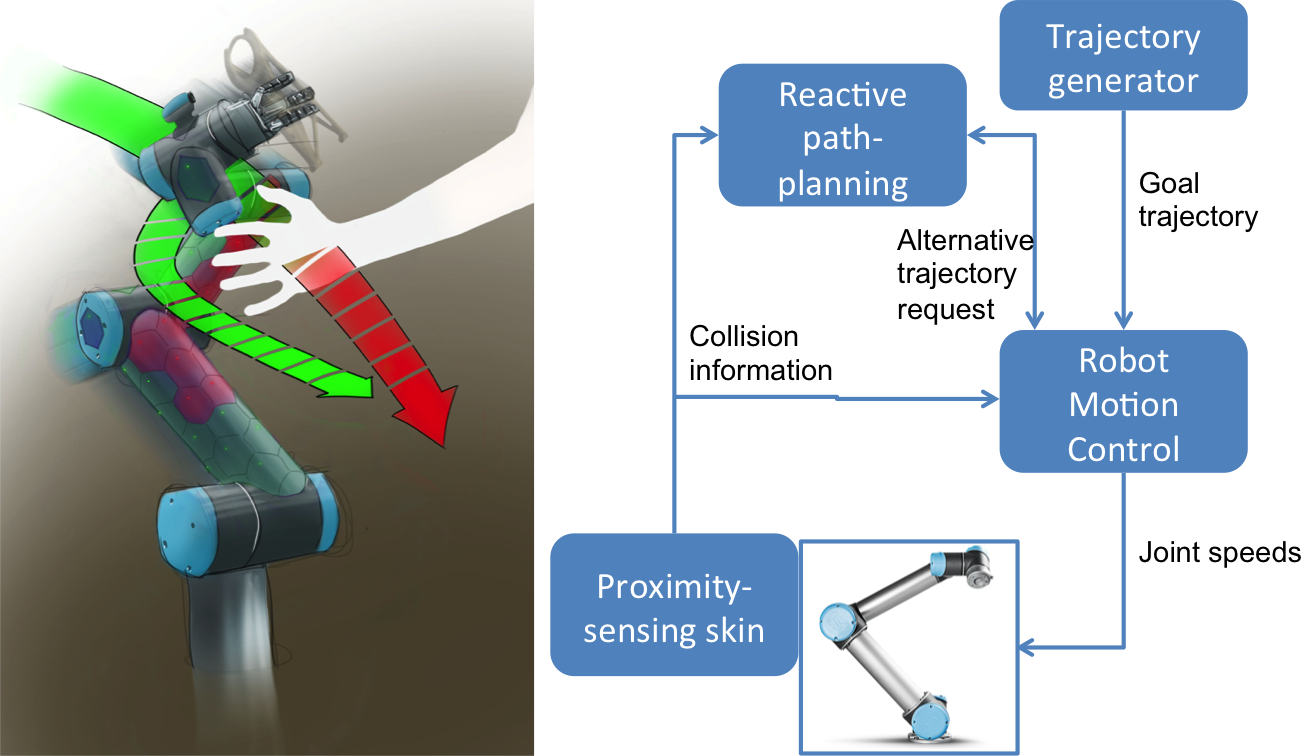
\includegraphics[scale=0.5]{chapters/doa/images/overview.png}}
\caption[0.1\textwidth]{An artist's schematization of the DOA
concept.}
\label{fig:overview}
\end{figure}
The figure \ref{fig:overview}(Left) shows the main idea of the framework which allows the robot arm to adapt its motion while executing a trajectory. The figure \ref{fig:overview}(Right) represents the pipeline of the framework used for collision avoidance and replanning. 
% \begin{figure}[h]
% \centering
% {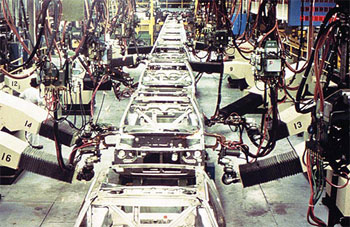
\includegraphics[scale=1]{intro/images/gm.jpg}}
% \caption{Manufacturing unit in General Motors with 'Unimate' robots in 1969}
% \label{fig:unimate}
% \end{figure}

\begin{figure}[h]
\centering
\resizebox{0.8\columnwidth}{!}{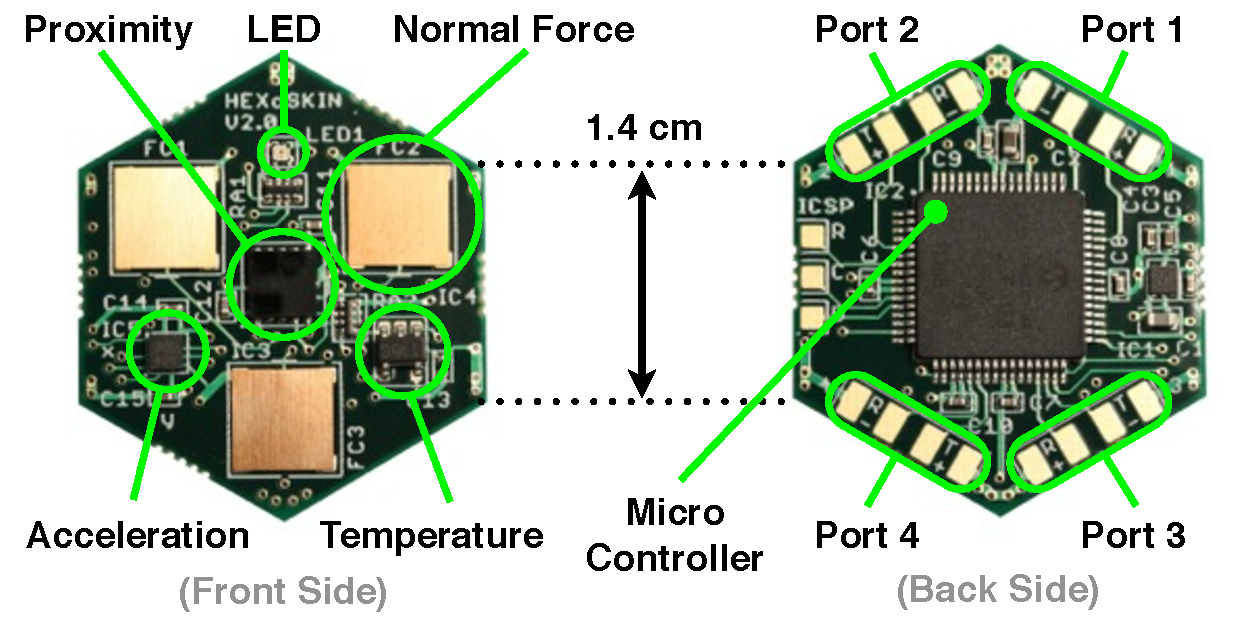
\includegraphics{chapters/doa/images/sensor_unit.pdf}}
\caption[]{Robot skin developed at Institute for Cognitive Systems, TUM.}
\label{fig:RobotSkin}
\vspace{-10pt}
\end{figure}	

\subsection{Artificial Robot Skin}
The development of \textit{Artificial Robot Skin}(ARS) is motivated by the necessity to provide robots with a rich and direct feedback of their interactions with the world. This system called as HEX-o-SKIN assembles multiple intelligent uniform unit cells with cell-2-cell communication allowing automatically cellular network organization \cite{mittendorfer2012uniform}. The robot skin system is modularized and transduces multi-modal tactile stimuli \cite{MittendorferYC15}. The robot skin consists of hexagonally shaped PCB modules called skin cells (see Fig. \ref{fig:RobotSkin}). A group of directly connected skin cells is termed skin patch. All skin cells are identical and contain the same set of sensors. The sensors sample 9 tactile stimuli of 4 different modalities, namely vibration (3D acceleration sensor), 3 normal forces (capacitive force sensor), 2 temperatures and 1 distance (optical proximity sensor). These sensors are either off-the-shelf standard ICs or in the case of the force sensors a in-house development. A micro-controller in the back of each skin cell collects data from its sensors, filters it and creates and sends data packets, which contain the most recent values of all sensors. All the skin cells are connected to each other via stretchable flex PCBs which allows the skin to cover curved surfaces and increases its robustness. The network of skin cells is a meshed bidirectional communication network which is routed by the micro-controllers of the skin cells. A self-organized algorithm initializes all the skin cells in a skin network and constructs a bidirectional communication path between each skin cell and the network root, the tactile section unit (TSU). The TSU converts skin network packets to standard UDP Ethernet packets and vice versa. This allows for fast low latency connections between robot skin and PC (see Fig. \ref{fig:SkinCellNetworkArchitecture}).
\begin{figure}[t]
\centering
\resizebox{0.8\columnwidth}{!}{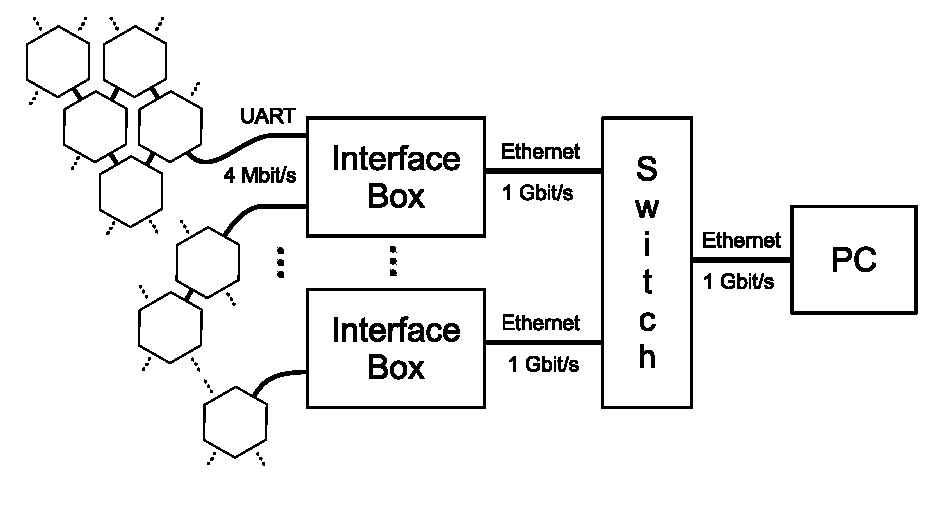
\includegraphics{chapters/doa/images/SkinCellNetwork.pdf}}\\[-15pt]
\caption[]{The skin cell network architecture and interface to the PC.}
\label{fig:SkinCellNetworkArchitecture}
\vspace{-10pt}
\end{figure}
The robot skin system also supports the auto-calibration of spatial relationships between skin cells of a skin patch covering a 3D surface \cite{Mittendorfer-IROS12tendorfer} such that the kinematic chain of every skin cell to the base frame can easily be determined. The proximity sensors used in the skin cells are infrared based sensors. The sensor emits infrared light and captures its reflections on obstacles in the range from 0 to 15 cm. The strength of the reflections allows the sensor to estimate the distance between the sensor and detected objects.  


\begin{figure}[h]
\centering
\resizebox{0.8\columnwidth}{!}{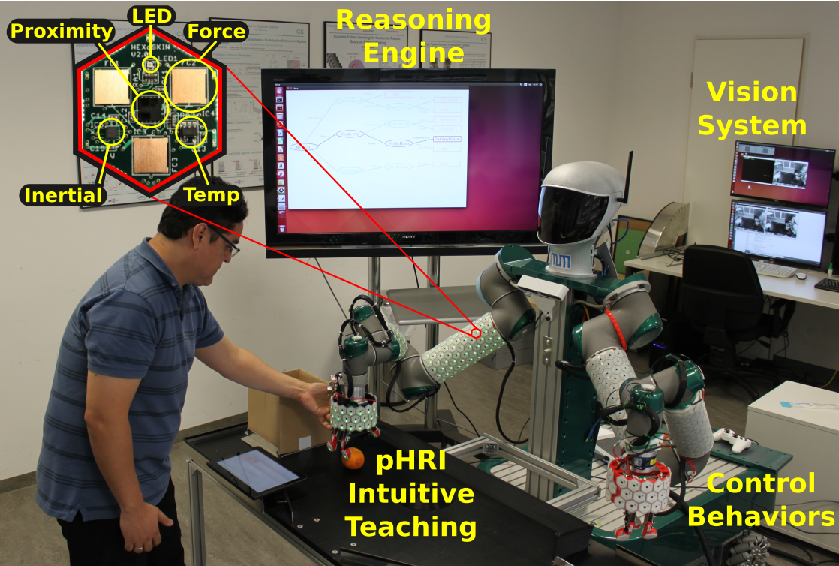
\includegraphics{chapters/doa/images/Demo.pdf}}\\[-10pt]
\caption[]{Robot TOMM with artificial robot skin.}
\label{fig:TommSorting}
\end{figure}

\paragraph{Evaluation of Artificial Robot Skin(ARS)}

The ARS has been successfully deployed on the robot TOMM \cite{Dean-ICRA17} (see Fig. \ref{fig:TommSorting}). The integration of the multi-modal artificial skin signals in the control loop of the arms is demonstrated in \cite{Dean-Humanoids16} where the self-calibrating artificial skin framework is used to control the dynamic behavior of the industrial robot, e.g. producing compliance in a non-compliant robot. The advantage of these compliant behaviors is to generate safer robots, especially for physical Human-Robot Interaction. The fusion of the multi-modal signals of the artificial skin with different sensors (e.g. cameras and joint encoders) in a semantic level is demonstrated in \cite{Ramirez-Amaro-Humanoids16}. These semantic representations are used to extract general task structures which together with the obtained knowledge can improve and accelerate teaching of new tasks \cite{Dynaov-Humanoids16}. Finally, the integration of these technologies has been evaluated in an industrial scenario, where a human can kinesthetically teach the robot TOMM to sort oranges \cite{Dean-IECON16} (see Fig. \ref{fig:TommSorting}). ARS has also been deployed successfully on another practical setup with a statically mounted Universal Robots UR5 robot (see Fig. \ref{fig:TUDSetup}). In this setup, the ARS is being used to provide proximity information related to obstacles in the immediate surroundings of the robot.

\begin{figure}[h]
\centering
\resizebox{0.8\textwidth}{!}{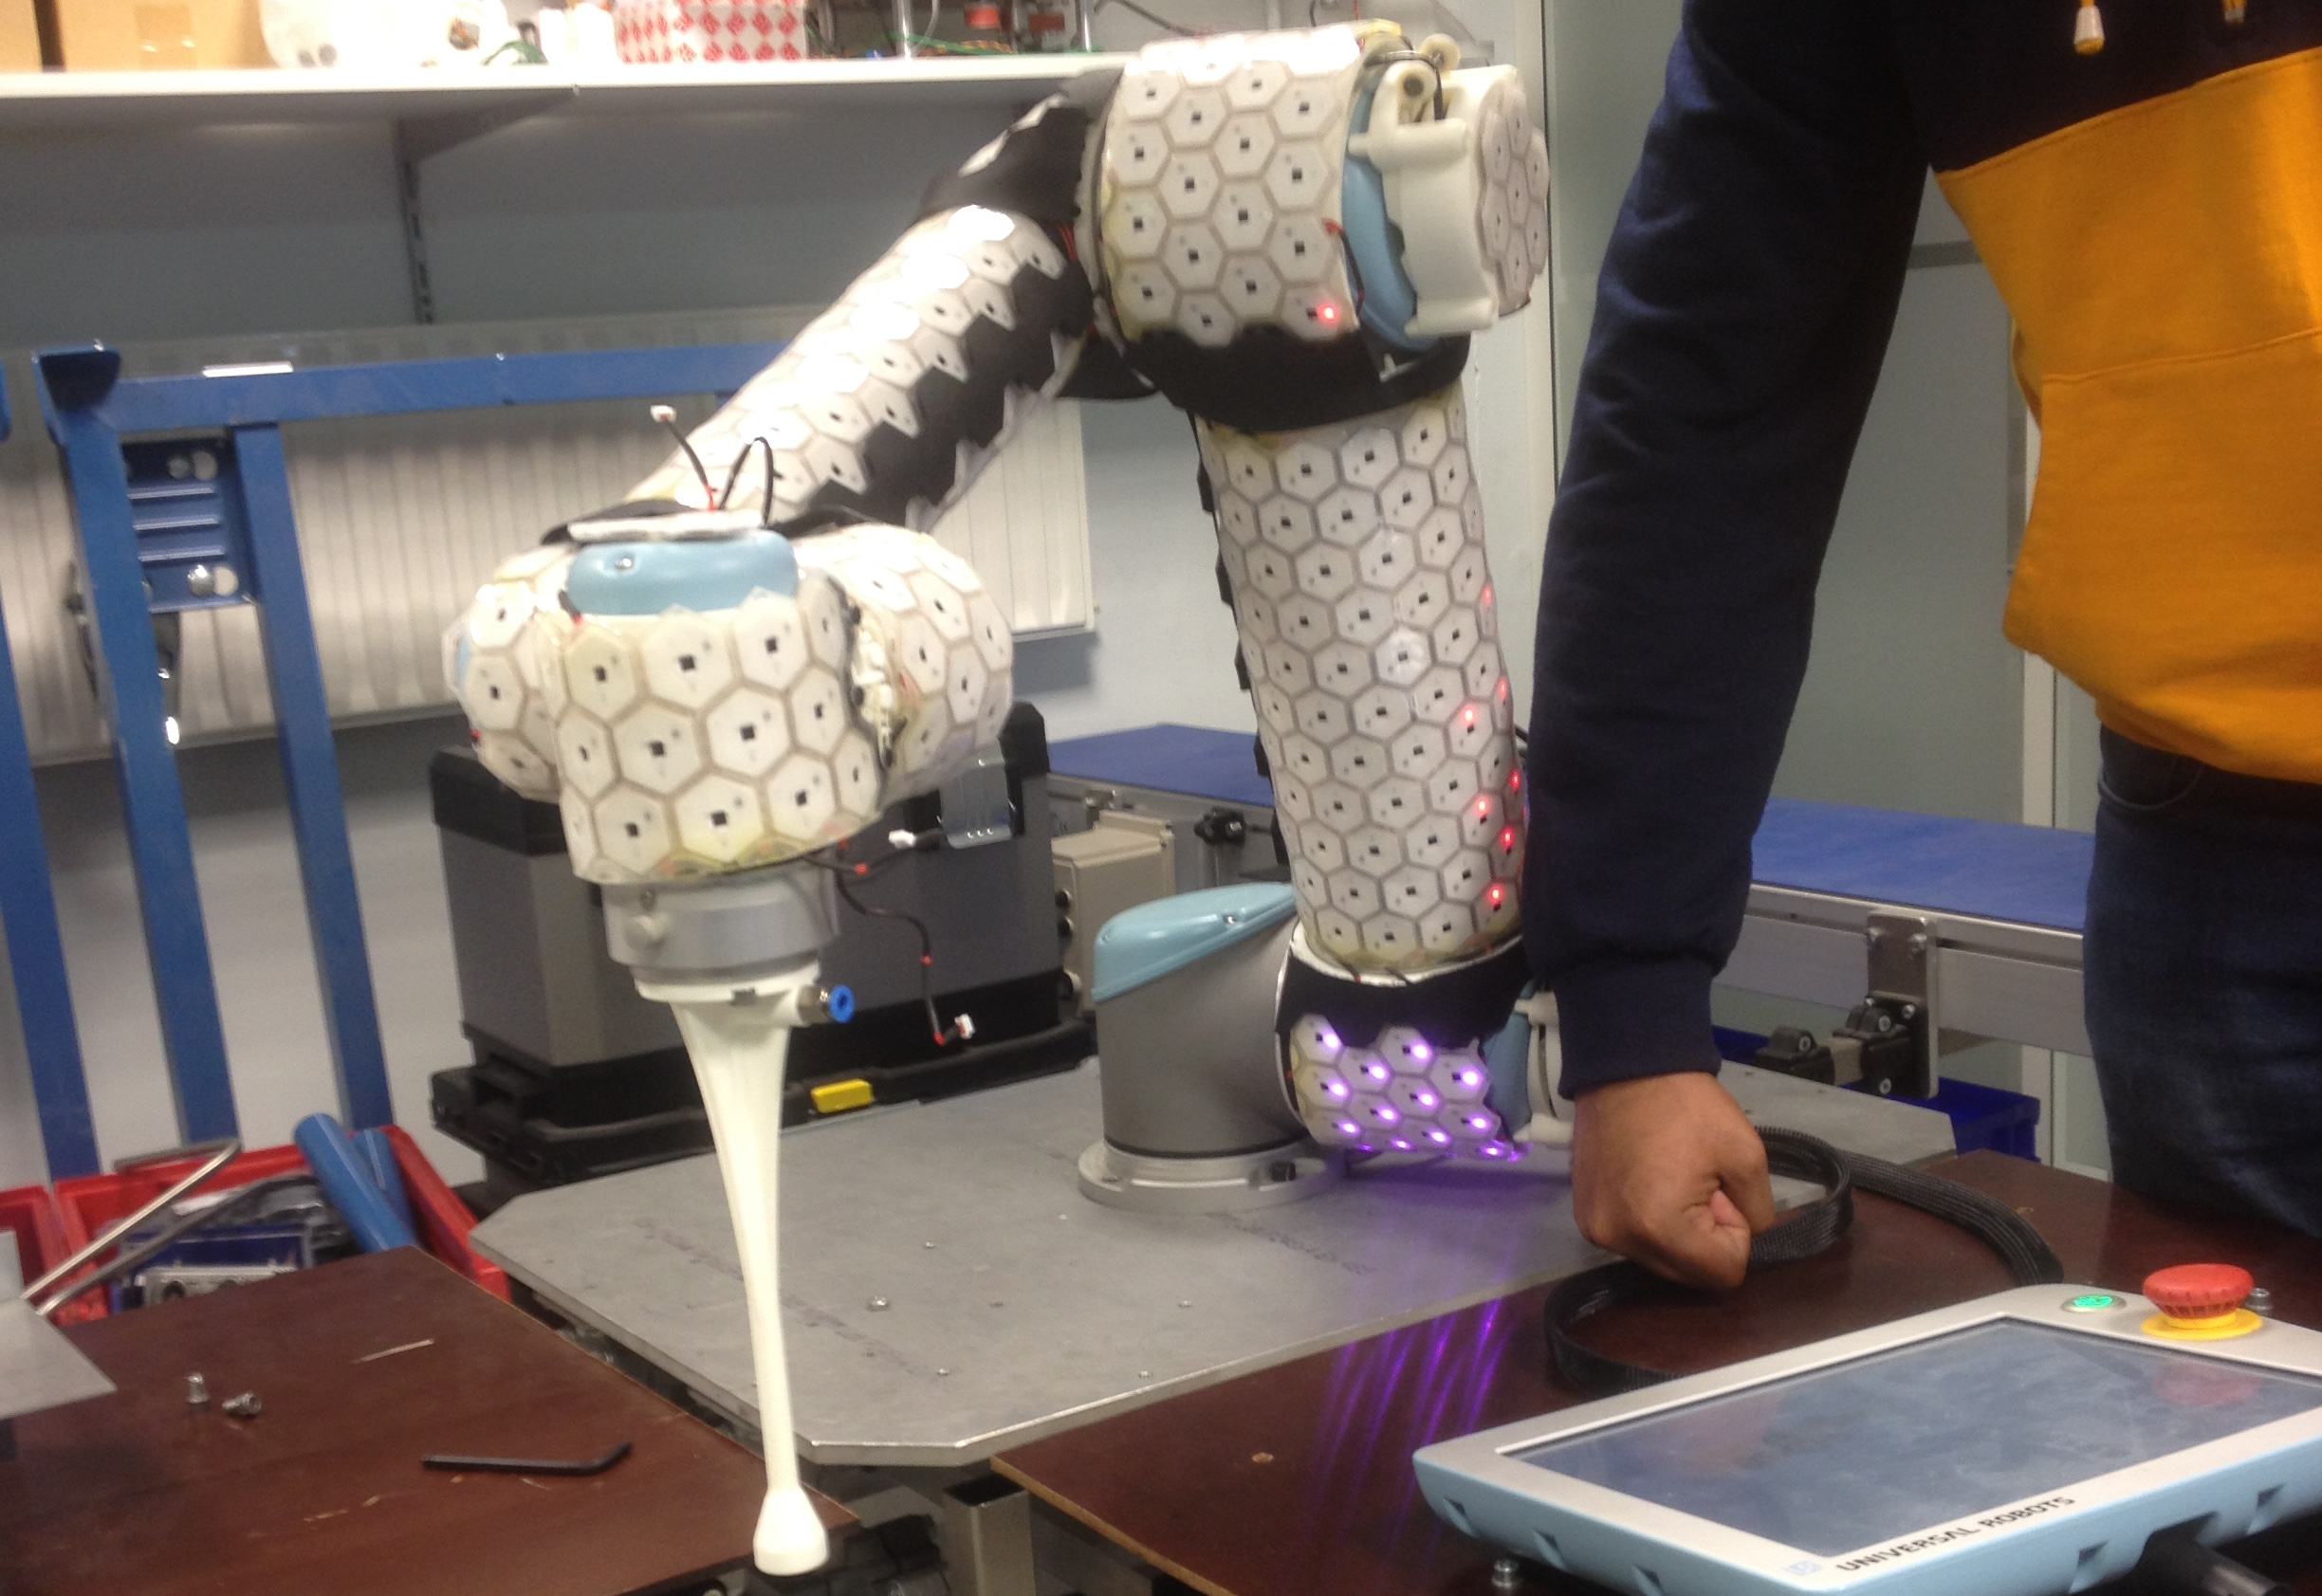
\includegraphics{chapters/doa/images/TUD_Setup.JPG}}\\[-10pt]
\caption[]{UR5 setup with Skin Cells activated (with red LEDs)}
\label{fig:TUDSetup}
\end{figure}


\subsection{Reactive Motion Planning}
\label{subsec:react_path}
\hypersetup{colorlinks, linkcolor=blue}
Though skin sensors can be used to reactively avoid obstacles locally, global aspect of the environment is necessary to avoid local minima, which is why we need an event based reactive replanner to help the controller in trouble. The reactive path planning component is developed by our partner Siemens, which is based on the industry grade KineoWorks\texttrademark\footnote{See
\href{http://www.plm.automation.siemens.com/en\_us/products/open/kineo/kineoworks/index.shtml}{Kineoworks}.} path planning library in order to provide fast and reliable robot paths. The intrinsic safety behaviors using torque/force sensing are reactive only after a collision has actually ocurred. This actually puts a constraint on the working velocity of the robot to be collaborative in industrial environments which we have pointed out earlier. The main motivation behind developing this component is to enable the robots to perform extrinsic safety behaviors which is quite inline with our goal to provide dynamic obstacle avoidance with appropriate caution. This component allows the robot to detect collisions in advance using depth information from Kinect camera and deform the trajectory by replanning in real time. The main advantage of using 3d sensors is to get a global view of the environment in contrast to proximity sensors on the surface of the robot which allows only local obstacle avoidance.

The complete collision avoidance component has been experimentally validated on a KUKA arm executing tasks in a environment with dynamic obstacles and a human operator. The reactive planner has been integrated with two trajectory generation frameworks: Reflexxes and Softmotion. Reflexxes \cite{kroger2011opening} framework can generate online time parameterized trajectories from a path. The generated jerk-limited and continuous trajectories takes into account of constraints on the dynamic robot capabilities with low latencies though there is no error bound between the reference and the executed trajectory.  The SoftMotion framework can generate online trajectories that limits jerk, acceleration and velocity for collaborative robot applications \cite{broquere2008soft,broquere2010motion}. The approach is based on the 7 segment acceleration profile by computing cubic curves for both point-point and continuous motions. The direct computation of the cubic parameters, the trajectory generator can be used on-line. Though it is incomplete as it cannot handle non-zero initial accelerations, it is experimentally validated and adapted for a KUKA LWR arm \cite{zhao2014online}. SoftMotion generates a trajectory with smoothing done at each stop point. The smoothed portion is constrained within a pre-defined tube respecting the error and kinematic bounds in real time making the trajectories more natural.



Actually, it is possible to use any trajectory generator as the planner generates a path as a polygonal line composed of a sequence of way points. For the proposed framework to avoid obstacles dynamically, we are only interested in the collision detection and the reactive planner module of this framework. The collision detection for dynamic obstacle avoidance is performed using the Kineo\texttrademark Collision Detector (KCD)\footnote{See \href{http://www.plm.automation.siemens.com/en\_us/products/open/kineo/collision-detector/index.shtml}{KCD}.}. KCD performs 3D collision detection and minimal distance analysis between triangular mesh surfaces in assembly environments. KCD has been designed specifically to minimize memory usage and take advantage of parallel processing. The component is synchronized with the OctoMap module which is updated at 30Hz with the point clouds acquired by an Xtion or Kinect camera sensors. Due to the necessity to perform reactive planning, the Octomap needs to be updated at higher rate which requires robust noise removal mechanisms. These filters removes Nan depth values and spurious points corresponding to noise, no-collision regions\& specular surfaces. The sparse outliers are removed using a statistical gaussian filter available in the PCL library \cite{rusu20113d}. The point cloud corresponding to robot links, joints and other bodies connected with the robot can be removed as well making the detection complete and flexible to be used in real time scenarios though the quality depends on a good hand-eye calibration.

\paragraph{Reactive path planning state machine}
Reactive path planning is done in the robot application node which coordinates the interaction between the path planning and the controller components executing the global tasks in real time. The path (re) planning strategy is implemented in the state machine as shown in the figure \ref{fig:KineoStates}.
\begin{itemize}
  \item \textbf{WAITING}: An idle state waiting for planning request.
  \item \textbf{PLANNING}: The controller requests the path planner node and waits for a collision free path composed of a sequence of way points. The controller executes a collision free trajectory by tracking the way points using Reflexxes or Soft Motion trajectory generator. In the proposed dynamic collision avoidance framework in the thesis, we use 'Stack of Tasks' to generate motions for a variety of reasons discussed in the next section.  In case the path planner fails due to nature of random tree algorithms, a fall back strategy to retry planning is implemented until a predefined timeout. The robot motion is cancelled in case no solutions exist.
  \item \textbf{MONITORING}: The trajectory execution by the robot is monitored for un-avoidable collisions. If the controller is intelligent enough to handle local collisions, the application node just monitors until the goal is reached. In case the obstacles doesn't allow for local path deformation, then the next state is triggered to replan.  
  \item \textbf{MONITORING WITH PLANNING PENDING}: An unavoidable collision is detected which has triggered to reach this state where the application node basically sends a new path planning request to the planner. Collisions are detected more accurately in this state as the reactive path planning considers the depth information represented in Octomap. The fast distance computation between the robot and environment using an efficient algorithm which is protected by Siemens, is used to reactively plan without creating any obstacle models which costs a lot of time.        
\end{itemize}

\begin{figure}[h]
\centering
\resizebox{1\textwidth}{!}{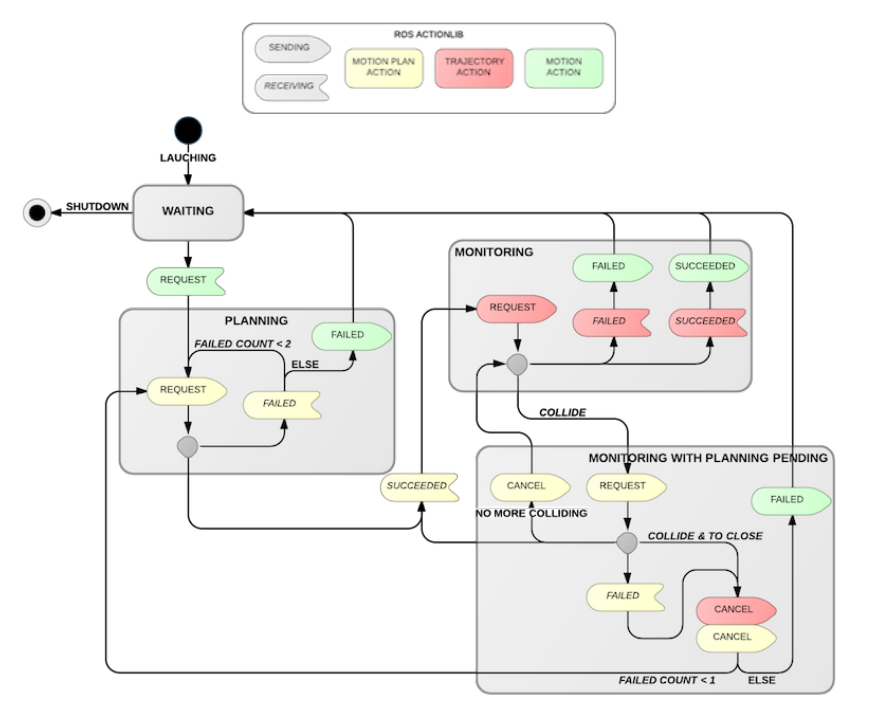
\includegraphics{chapters/doa/images/kineo_0.png}}\\[-10pt]
\caption[]{Reactive Path Planning State Machine}
\label{fig:KineoStates}
\end{figure}

This framework has been seamlessly integrated into the ROS-ecosystem via a ROS package called \texttt{kws\_ros\_interface} which provides the planner implementations of KineoWorks as shared objects that are readily usable in ROS-based software via the \texttt{kws\_ros\_planner} ROS node.Robot kinematic models are provided to KineoWorks in the Unified Robot Description Format (URDF) which is a ROS standard. Furthermore, KineoWorks also accepts the standard ROS representation of a \texttt{PointCloud}\footnote{See http://wiki.ros.org/pcl} for creating collision models of dynamic obstacles in the environment. 

\subsection{Reactive Controller}
The complete software architecture used for the Dynamic Collision Avoidance capability is shown in Fig. \ref{fig:arch_dca}. The motion control is achieved using the Stack of Tasks (SoT) controller framework \cite{Mansard2009} which employs a task based hierarchical jacobian control strategy eliminating the analytical inverse kinematics computation thus making it a generic controller for all robot platforms. 
The task function formalism is very well discussed in \cite{C.Samson1991}. A \emph{task} basically is a control law that achieves a specific objective which can be a free space task or just an inequality constraint that narrows down the workspace of the robot. The controller's hierarchical nature allows the robot to handle multiple kinematic tasks simultaneously exploiting the kinematic redundancy of the robot. The controller's real time capability comes from the high computational speed of the state of the art Hierarchical Quadratic Programming (HQP) solver backing it. In the context of our work, tasks generally include robot joint posture task, collision avoidance task, joint limits task and so on. The SoT framework handles the task priorities hierarchically in the real time to ensure there are no conflicts among tasks which is used to achieve dynamic obstacle avoidance without compromising on the main goal.

For example, let us consider a pick and place application in a collaborative environment. The primary goal for this application is to enable a robot to move to a (set of) desired pick and place locations repetitively. The pick and place locations can be defined as posture tasks in SoT. However, a higher priority task considering the collaborative nature of the environment is to avoid
collisions with obstacles that could be humans, for instance. Typically such a task is modelled as an ``Inequality'' task and an eventual feasible solution (if one exists) is computed by the solver by exploiting the kinematic redundancy of the robot. In the jargon of motion planning and control, this behavior is similar to a \emph{local planner}. However, it is likely that a feasible solution is not found due to the solver converging to a local minima\footnote{This is caused by the use of task Jacobians. For further details, please see \cite{Mansard2009}.} In such a scenario, SoT can also be used to leverage the services of a global planner (see Section \ref{subsec:react_path}) from the current robot state to the goal so that an entirely new path is obtained which is free from collisions and consequently allowing all the specified tasks to be achieved in the order of their priorities. The SoT controller has also been configured to work with the ROS-control interface. In all these setups, the proximity information from the artificial robot skin is used as an input to the collision avoidance task. In the following part, we briefly present the global path planner software framework that is used when the SoT controller hits a local minima.
\begin{figure}[t]
\centering
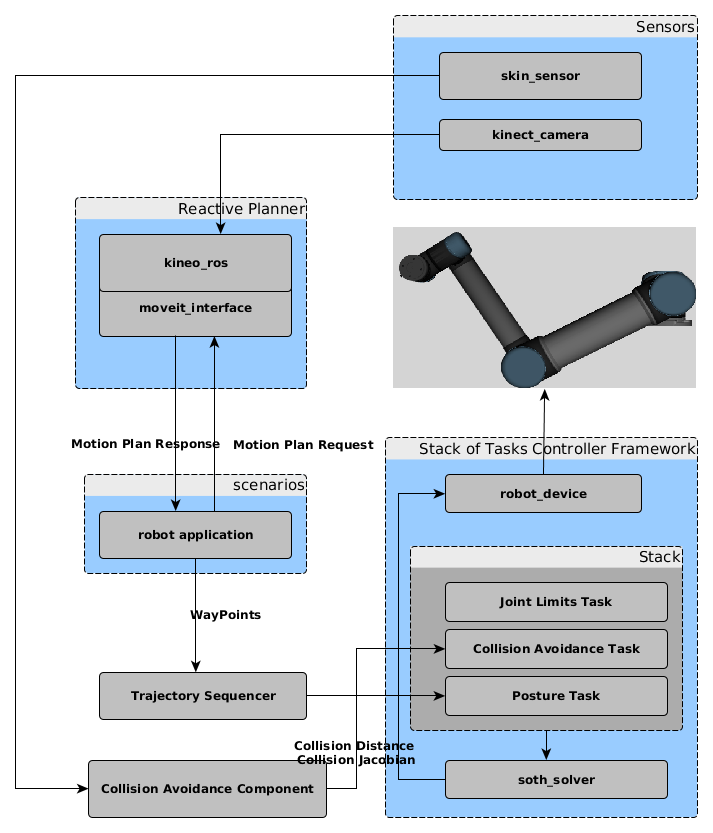
\includegraphics[scale=0.47]{chapters/doa/images/arch_dca.png}
\caption[]{Dynamic collision avoidance software architecture.}
\label{fig:arch_dca}
\end{figure}

\section{Reactive Collision Avoidance using SOT}
\label{sec:sot}
'Stack of Tasks' is a hierarchical jacobian-based task controller framework which implements the generalized inverse kinematic formalism by Hanafusa et Al. for local control of redundant systems\cite{hanafusa1981analysis}\cite{Mansard2009ik}. The framework in the earlier stages implemented the Siciliano's extension to handle multiple equality tasks\cite{siciliano1991general}. It has evolved to handle inequality constraints implementing the state of the art solver. The framework provides a structure that orders actives tasks to compute the control law without compromising on the task priority and control continuity. The framework provides a simple scripting interface to interact with controller components during the runtime and has a wrapper to communicate with the ROS world.
\subsection{State of the Art}




%    \begin{figure}[thpb]
%       \centering
%       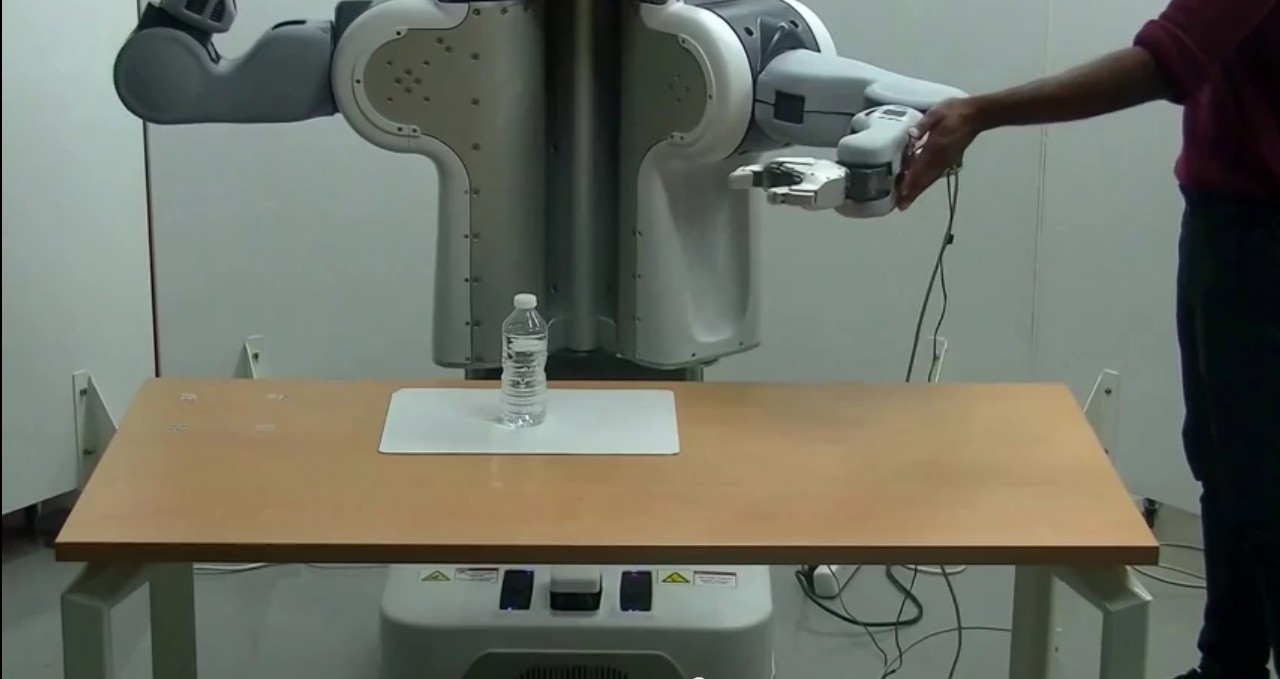
\includegraphics[scale=0.2]{chapters/doa/images/skin.eps}
%       \caption{A mobile manipulator executing a trajectory to reach a pre-grasp pose while the forearm is approached by a person with his hand. A skin sensor mounted on the forearm is used to sense any obstacle in the proximity. }
%       \label{figurelabel}
%    \end{figure}


Morover  redundant systems are popular due to their increased flexibility of arm and a mobile base to handle inequality constraints. The control of redundant robots is not trivial as it is not always easy to compute  analytic inverse kinematic and dynamic solutions. Task function based approach  resolves redundancy to minimize the error in task space \cite{Samson1991}. They are jacobian based techniques inverting the differential mapping that maps the control space and the error space to compute optimal controller outputs. A systematic framework for redundant system control proposed by Siciliano allowed to execute multiple tasks simultaneously with priorities {siciliano1991general}. These framework can only solve equality tasks and various strategies focuses on transforming inequality constraints to equalities\cite{Nelson95strategiesfor,chan1995weighted,mansard2009directional,raunhardt2007progressive}. These strategies are not generic enough and has priority inversion problems making them unreliable for practical use. 

A cascade approach was alternatively used to represent the inequalities and equalities systematically as a hierarchical least square program[Kanoun 2011] but suffered from computational inefficiencies. Hierarchical quadratic program (HQP) solver uses complete orthogonal decomposition (COD) instead of singular value decomposition (SVD) and an improved search algorithm which makes it more efficient than available solvers \cite{escande2014hierarchical}. Though constraint based approaches are quite an efficient way to handle collisions and a flexibile way to model them, the are merely locally optimal controllers and does not provide a systematic way to escape local minima. This necessitates the support of global path planners to find the optimal path for realizing a robot task. Combining global path planning and a reliable reactive control is an essential need for deploying robots from simple to complex scenarios.

 
\subsection{What is a Task?}
A task basically composes a control law with a specific objective which can be such as reaching a desired joint position, avoiding obstacles in the environment, a visual servoing mechanism for grasping or so on. A task is mainly defined by the error between the desired and current feature, the error jacobian and the gain. These defined tasks are pushed into 'Stack of Tasks' which computes the control law for all the task objectives in an iterative manner\cite{mansard2007task}. 

\[\textit{e(t) = x\textsuperscript{*} - x }\]

where \textit{x} refers to the current state of a feature, \textit{x\textsuperscript{*}} refers to the reference feature.

\subsection{Redundancy Formalism}
Siciliano and Slotine proposed a systematic control framework to compute controller outputs for achieving multiple tasks in redundant systems from the redundancy formalism proposed by Hanafusa et al. The idea is, tasks are solved only in the null space of the higher priority tasks to avoid conflicts with them. This means, a task at any level has no effect on the tasks in the higher level as it uses only the left degrees of freedom. 

Let $(e_{1},J_{1})$ be a primary task  which is defined by  
\begin{equation} \label{eq:tf1}
\dot{e} = J\dot{q} 
\end{equation}
 \textit{J} referring to the Jacobian of the error velocity with respect to joint velocity at the current joint state.


\begin{equation} \label{eq:tf3}
\dot{q} = J_{1}^{+}\dot{e}_{1} + Pz
\end{equation}
 Where \textit{P} is the projector on the null space of the the Jacobian J and \textit{ $z$ } is the arbitrary velocity vector which can be used as a parameter to achieve the secondary objectives. 

Let $(e_{1},J_{1})(e_{2},J_{2})...(e_{n},J_{n})$ be tasks in the stack. The redundancy formalism for two tasks can be extended to n tasks such that $e_{i}$ does not conflict with $e_{j}$ such that $j<i$. 


The recursive joint velocity is of the form
\begin{equation} \label{eq:ntasks}
  \dot{q}_{0} = 0\\
\end{equation}
\begin{equation}
  \dot{q}_{i} = \dot{q}_{i-1}+ (J_{i}P^{A}_{i-1})^{+}(\dot{e}_{i} - J_{i}\dot{q}_{i-1}), i= 1..n
\end{equation}



 where $P^{A}_{i-1}$ is the projector onto the null space of the augmented Jacobian $J_i^A = (J_1...J_i)$ and $\widetilde{J}_i = J_iP_{i-1}^A$ is the limited jacobian of the task. The joint velocity achieving all the task objectives is $\dot{q} = \dot{q}_n$. The recursive projector is computed by 
 
 \[P^A_i = P^A_{i-1} - (J_iP_{i-1}^A)^+J^A_{i-1}  \] 
 
 This systematic way of prioritizing tasks allows simultaneous execution of multiple tasks without conflicting each other.
 \subsection{Hierarchical Quadratic Programming}
Mansard et al. proposed an improved QP solver to manage multiple equality and inequality problems in a prioritized hierarchy to handle redundancies[15]. The solver handles equality tasks quite the same like in Siciliano's framework but the solver uses complete orthogonal decomposition(COD) instead of Sing for solving the least squares which is quite faster and efficient. The Hierarchical complete orthogonal decomposition(HCOD), a COD of the jacobian mapping for all the levels is used to compute primal optimum for all the constraints at once making it computationally faster. 

Kanoun et al. and De lasa et. al used a primal active search algorithm which is very expensive due to inefficient optimal active set search involving inappropriate activation and deactivation of constraints at each level along the cascade\cite{de2010feature}\cite{kanoun2011kinematic}. The HQP solver depends on a modified primal active search algorithm to make the optimal active set computation much more efficient. Lexicographic optimization formalism is introduced to maintain the active set at each iteration consistent with prior levels completely eliminating unnecessary constraint deactivations and activations. The solver is ten times faster than the classical solvers and can consider inequalities at any levels of the
hierarchy \cite{escande2014hierarchical}.

\subsection{Collision Avoidance using SOT}
   \begin{figure}[thpb]
      \centering
      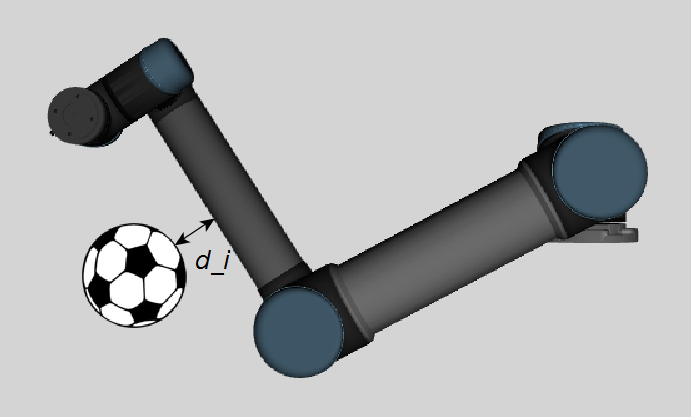
\includegraphics[scale=0.5]{chapters/doa/images/robot-obstacle_raw.png}
      \caption{Robot-Obstacle Interaction }
      \label{gso}
   \end{figure}
\subsubsection{Collision Avoidance Task Formulation}
Suppose an obstacle in the environment is close to the vicinity of the skin sensors on the robot less than a safe margin (or) threshold, the robot can move orthogonal to avoid potential collisions. Consider a multi-body robot with $n_c$ skin cells $\mathcal{C}_1,\mathcal{C}_2,\mathcal{C}_3 ... \mathcal{C}_{n_c}$ on the surface of the links. Let us also represent $\mathcal{C}_i(q)$ to be the position of the cell on the robot body  at a robot configuration q and the environment obstacle as $\mathcal{O}$. The range information from the sensors are basically the proximity distance between the skin cell and the environment obstacle in the vicinity represented by $d_i(q)$ at a robot configuration q. The below formulation is an alternative to potential field which is as follows:   
\begin{equation} \label{eq:d_ineq} 
d_i(q)  >= d_{min}
\end{equation}

Refactoring:
\[ (d_{min} - d_i(q))  <= 0\] 
\begin{equation} \label{eq:d_ineq} 
f_i(q)  <= 0
\end{equation} 

where $ f_i(q) = (d_{min} - d_i(q))$
\newline
We model an Ordinary differential inequality for the distance inequality constraint to use it in the SOT solver working in the kinematic level. 

\begin{equation} \label{eq:dd_ineq} 
\frac{\partial f_i(q) }{\partial q} \dot{q} <= - K f_i(q)
\end{equation} 

where: K is the convergence gain\newline
This formulation allows for an exponential convergence of the modeled inequality task. In our case after refactoring, \ref{eq:dd_ineq} zeros down to below form

\begin{equation} \label{eq:solver} 
-\frac{\partial d_i(q) }{\partial q}  \dot{q} <= -K (d_{min} - d_i(q))
\end{equation} 

\begin{equation} \label{eq:final} 
\dot{d_i(q)} >= K (d_{min} - d_i(q))
\end{equation}
\subsubsection{Proximity Distance Gradient Computation}
The computation of the gradient of the proximity distance between the collision bodies inspired from \cite{lefebvre2005fast} is required to define inequality constraints in Stack of Tasks to avoid self-collision and with external obstacles using a proximity sensor.

\begin{equation} \label{eq:proxd}
d_i(q) = d(\mathcal{C}_{i}(q),\mathcal{O}) = \|\mathcal{O} - \mathcal{C}_{i}(q) \|
\end{equation}
The gradient of the above distance with respect to the robot configuration is given by:

\[ \frac{\partial d_i(q) }{\partial q} = n.(\frac{\partial \mathcal{O}(q) }{\partial q}-\frac{\partial \mathcal{C}_{i}(q) }{\partial q}) \] 

where: 
\[ n = \frac{(\mathcal{O} - \mathcal{C}_{i}(q))^T}{ \|\mathcal{O} - \mathcal{C}_{i}(q) \| }\]

Assuming the environmental obstacle to be static because of the inability to measure the differential change, the gradient boils down to the below form.

\begin{equation} \label{eq:proxdiff} 
\frac{\partial d_i(q) }{\partial q} = -n.\frac{\partial \mathcal{C}_{i}(q) }{\partial q}
\end{equation}

 







% \subsection{Proximity Distance Gradient for Collision Avoidance}
% The computation of the gradient of the proximity distance between the collision bodies inspired from \cite{lefebvre2005fast} is required to define inequality constraints in Stack of Tasks to avoid self-collision and with external obstacles using a proximity sensor. Let $d$ be the distance between approximated collision bodies $O_1(q)$ and $O_2(q)$. The distance between these bodies and its variation is mapped to joint actuations $q$. The distance gradient can be computed by:
% \[ \frac{\partial d}{\partial q} = n_d^{'}(\frac{\partial o_1(q)}{\partial q}- \frac{\partial o_2(q)}{\partial q}) \]

% where $n_d^{'}$ is the unit normal distance vector while $o_1(q)$ and $o_2(q)$ are the respective closest points. The gradient of the closest point $p$ of fixed coordinates $(\rho_1(q),\rho_2(q)....\rho_l(q))$ in the local reference frame $(e_1(q),e_2(q)...,e_l(q))$ of a collision object at joint configuration $q$ is

% \[\frac{\partial p}{\partial q} =  \sum_{l=1}^{d}\rho_l(q)\frac{\partial e_l(q) }{\partial q}\]

% In a 3 dimensional workspace, the expression can be written as 

% \[ \frac{\partial p}{\partial q} =  (x y  z)J_\omega + J_\nu \]

% where $J_\omega$ is the jacobian of the rotational degrees of freedom $J_\nu$ is the jacobian of the linear degrees of freedom. In case of the external objects, the second part of the equation can be eliminated if the object is static. 

% This work is a direct application of the HQP solver and a first attempt to combine path planning and reactive control in a jacobian based solver framework eliminating a cumbersome architecture handling the information flow between control and planning components. Stack of Tasks, a controller framework that implements the latest HQP solver is used in this work to apply the proposed methodology. The proposed methodology is tested on PR2, a mobile manipulation platform with a skin sensor mounted on the forearm of the robot to demonstrate the collision avoidance while executing a planned trajectory without compromising the final goal of the scenario. 


% The paper is organised as follows. Section \ref{sec:application} describes the solution for dynamic obstacle avoidance and Section \ref{sec:skin} discusses the proximity-sensing robot skin. In Section \ref{sec:sot} the robot motion control architecture to incorporate the collision information as safety
% constraints to dynamically adapt the trajectory is presented. Section \ref{sec:prelim_results}
% presents the preliminary results obtained in two different robot setups. Finally, in Section \ref{sec:conclusions} we present our concluding remarks and a discussion of the current work in progress.




\paragraph{Combining Path Planning and Reactive Motion Control}

The methodology is based on defining the main goal as a workspace constraint and prioritizing between safety tasks and trajectory execution task (in joint space). The figure \ref{gso} gives an intuitive idea about the stack priority order.

   \begin{figure}[H]
      \centering
      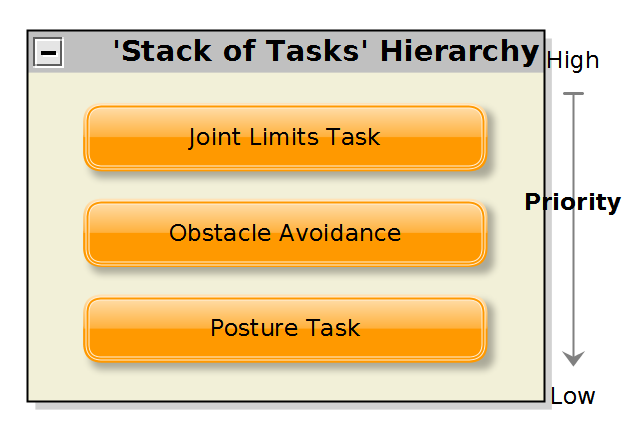
\includegraphics[scale=0.5]{chapters/doa/images/sot_hierarchy.png}
      \caption{Generic stack order for combining planning and control. }
      \label{gso}
   \end{figure}
   \begin{itemize}
  \item[T1] Obstacle Avoidance
  \newline
\hspace*{0.1cm}$\dot{d_i(q)} \geq \lambda_{1}(d_{min} - d_i(q))$\newline
\hspace*{0.11cm}where $d_{min}$ is the safety threshold
  \item[T2] Posture Task
  \newline
\hspace*{0.1cm}$\dot{q} = q_{ref} - \lambda_{2}(q-q_{ref})$\newline
\hspace*{0.1cm}where $q_{ref}$ is the reference trajectory
\end{itemize}
SOT controller computes $\dot{q}$ in order to satisfy T1 and T2 (at best)



% Safety tasks are obviously given higher priority in the stack for collision avoidance. Trajectory execution in Joint space occupies the least priority which leaves the controller only the left degrees of freedom from the primary task. If a joint trajectory crosses an unforeseen or dynamic obstacle and if the sensors can sense it, the robot basically cannot execute the trajectory until the object is actually moved out of its way. Replanning could be activated if there is no other possibility to reach the joint trajectory goal. Even if there is a possibility to avoid the obstacle and continue executing the trajectory, it is always not sure that the robot will end up in the desired goal in the task space. The clever trick here is in the way the main goals are defined. The main goal can be moving a base to a particular pose in the world or move the end effector to a grasping pose. Here the important thing is that the goals are something defined in the workspace though a joint trajectory is executed to achieve them. The hierarchical nature of the controller puts this main goal task in high priority and the jacobian core of the solver finds an optimal solution to follow the main goal. The next section illustrates this methodology on a simple scenario to show the potential of this method.



\section{Experimental verification of Reactive Collision Avoidance}
The Stack of Tasks (SoT) controller with collision avoidance constraints has also been deployed and tested for achieving different postures on the setup in Fig. \ref{fig:TUDSetup}. We have integrated the behavior to path following with the reactive collision avoidance as shown in Fig. \ref{fig:dca}. Though it is integrated, we consider these presented results preliminary yet quite convincing to be go in this direction to develop a reactive collision avoidance technology.

\subsection{Experiments in a mobile robot - PR2{\color{red}  (to be updated)}}

The framework was very initially tested with the given skin cell prototype on PR2, a mobile robot. The skin patch with eight cells is stuck on the arm to sense proximity range information. A simple manipulation scenario is executed and getting close to the arm sensors induced base motion to avoid obstacles while still executing the trajectory. The experiment can be seen here in this \href{https://youtu.be/y-6Oyi21ioQ}{\textcolor{blue}{video}} and the snapshots are shown in this Fig \ref{fig:pr2avoid}. The graph \ref{fig:basegraph} shows the evolution of the robot base when it encounters an obstacle. The safe region is where the skin cell - obstacle distance is within the right limits ensuring safety. Although the base goes away from the obstacle, it recovers back to its previous or commanded pose in the trajectory. 
\begin{figure}[ht]
\centering
\begin{subfigure}
[Getting close to the arm]{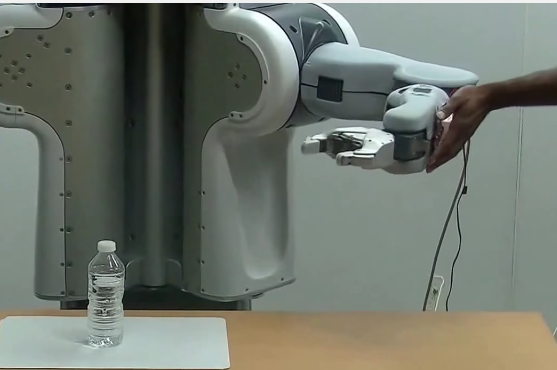
\includegraphics[width=5.5cm,height=6cm]{chapters/doa/images/pr2_0.png}}
\end{subfigure}
\begin{subfigure}
[Base motion to avoid the obstacle]{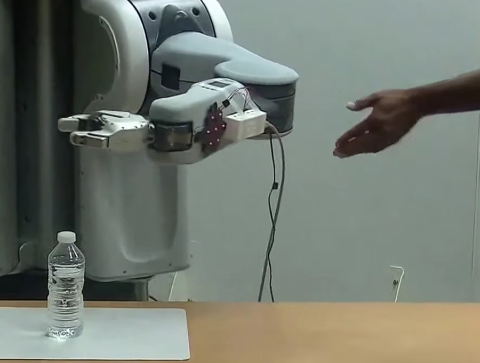
\includegraphics[width=5.5cm,height=6cm]{chapters/doa/images/pr2_1.png}}
\end{subfigure}
\caption{Obstacle Avoidance in PR2 using skin prototype}
\label{fig:pr2avoid}
\end{figure}

\begin{figure}[!ht]
\centering
{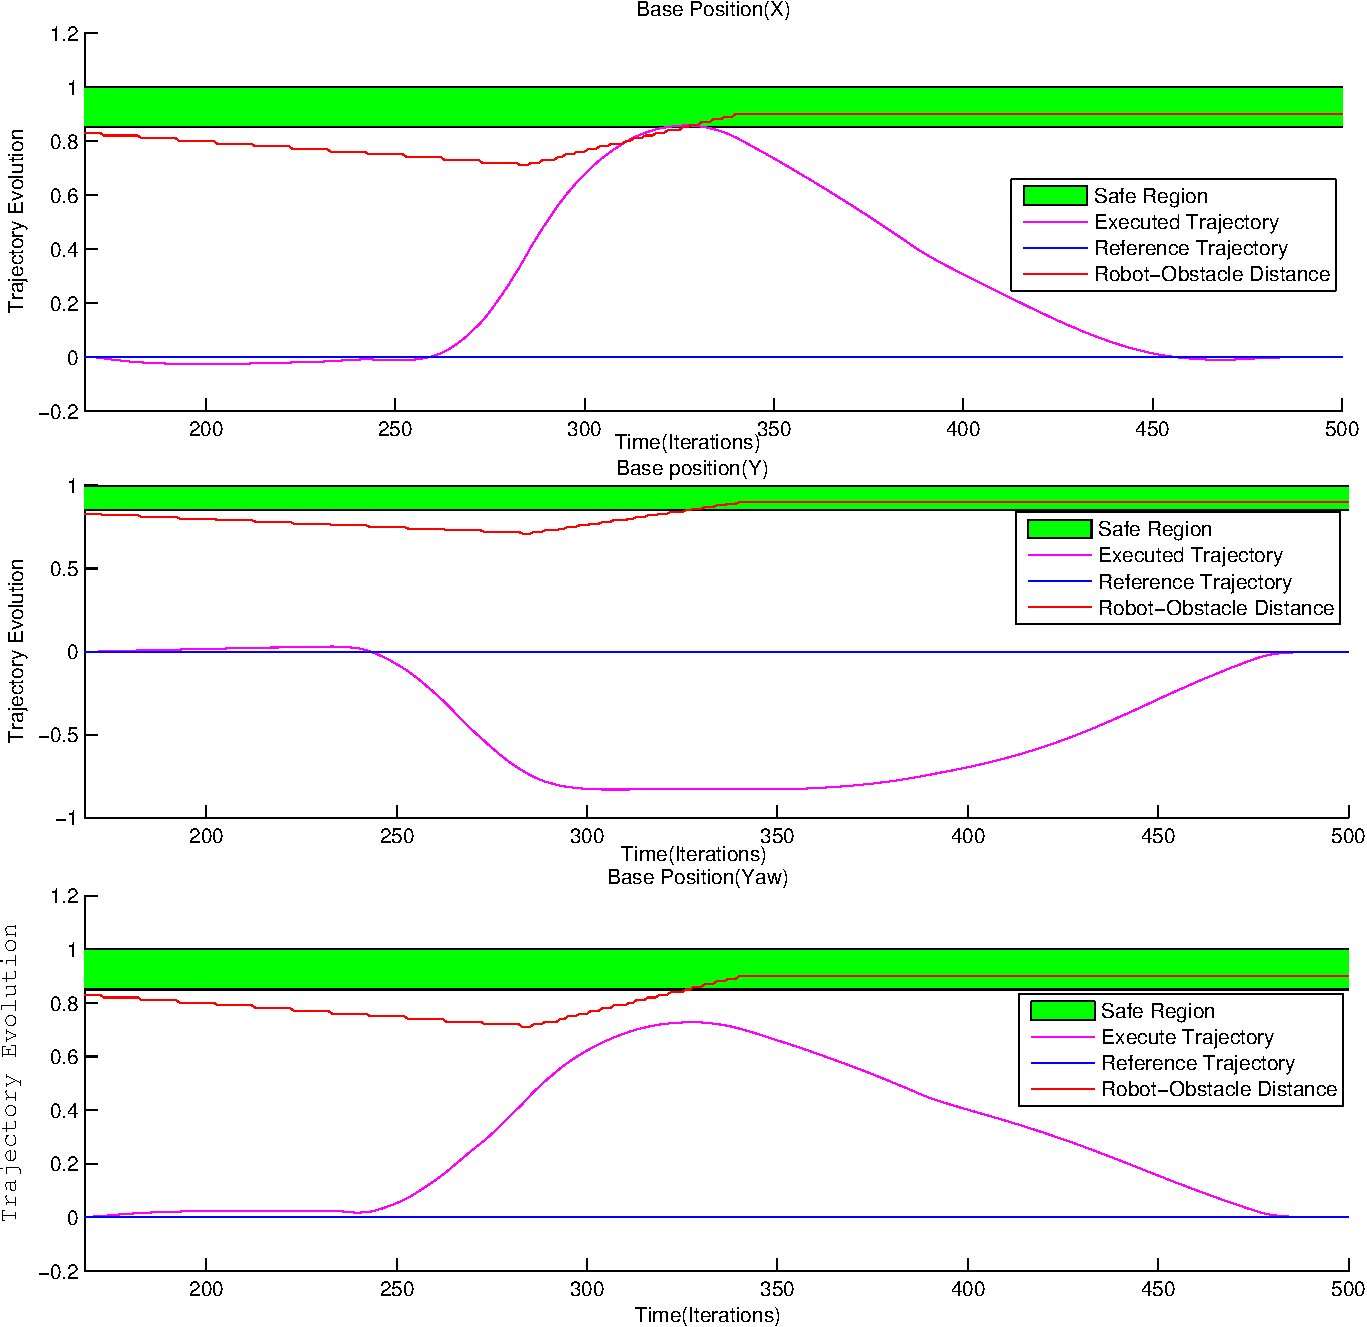
\includegraphics[scale=0.5]{chapters/doa/images/baseplot-crop.pdf}}
\caption{Base Position Evolution}
\label{fig:basegraph}
\end{figure}




\subsection{Experiments with Reactive Replanning in TOMM Setup}
\hypersetup{colorlinks, linkcolor=blue}
The integration of all the components described earlier has been evaluated on a simulation of the orange sorting setup as shown in Fig. \ref{fig:TOMMSimulation}. The evaluation is done in a ROS based gazebo environment with the skin sensors simulated using the flexible collision library to project the distance between objects to sensor range measurements. These measurements are mapped to signals compatible in dynamic graph framework using a bridge component to allow its use in the SoT controller. The reactive planning component having the capability to plan with point cloud data using a Moveit python interface to query motion plan requests. 
\begin{figure}[ht]
\centering
\resizebox{0.85\columnwidth}{!}{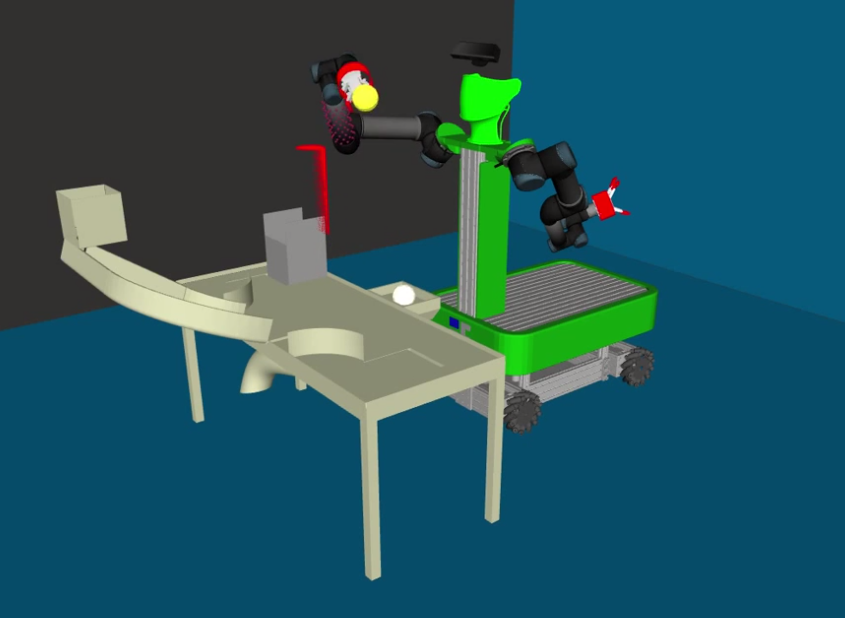
\includegraphics{chapters/doa/images/tomm_simulation.png}}\\[-10pt]
\caption[]{Orange sorting scenario in simulation.}
\label{fig:TOMMSimulation}
\end{figure}
The combined use of a reactive motion planner and a hierarchical reactive SoT controller with skin data makes it a good candidate for applying dynamical obstacle avoidance in factory environments. A video result of the same is available \href{https://youtu.be/uLStjR7mpOI}{\textcolor{blue}{here}}. Though it is tested in simulation, an experimental verification on a real robot setup with 3d cameras is quite essential to qualify the proposed framework as a promising technology. But the collision avoidance is tested on a UR robot with skin sensors to verify the local reactivity of the controller. 

\subsection{Experiments in a UR5 robot}

\begin{figure}[H]
\centering
{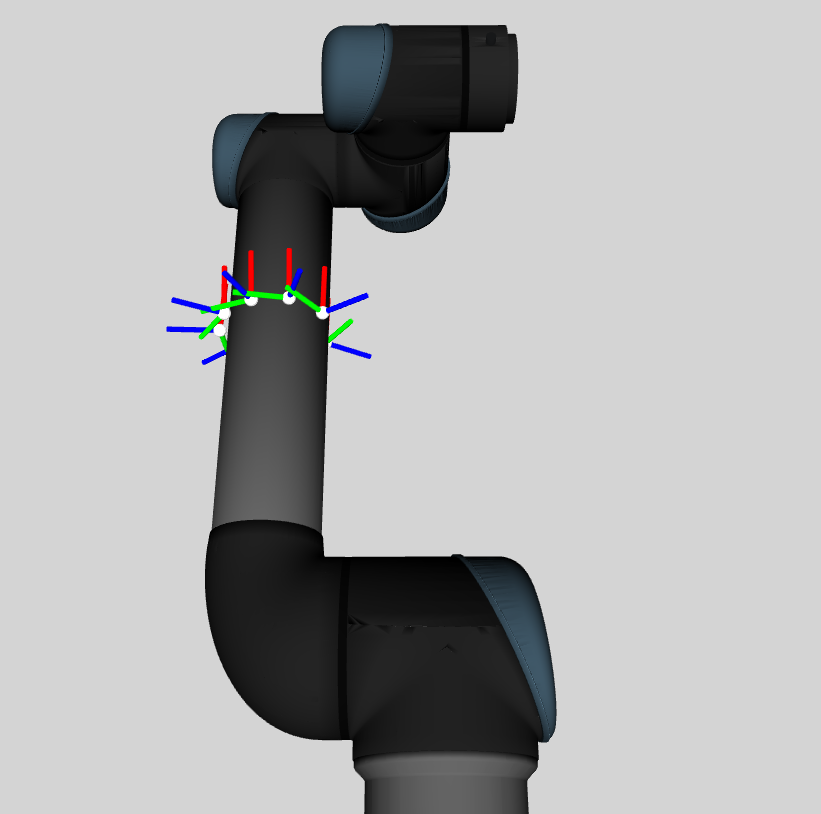
\includegraphics[width=6.5cm,height=6cm]{chapters/doa/images/delft/ring_sensors.png}}
\caption{Sensor Ring on the Upper Arm}
\label{fig:ringsensors}
\end{figure}

The reactive collision avoidance is experimentally verified on the UR5 robot with the skin sensor setup. The skin sensor network  consists of approximately 300 cells in total covering the entire surface of the UR5 robot arm. Though it is interesting to model all the skin cell constraints to be resolved by the controller, it is practically impossible to solve all the inequality constraints using the current state of the art solver due to computational constraints. A proper approximation is necessary to minimize the number of inequality constraints fed to the solver at every control cycle. In the set of preliminary experiments conducted, we defined a skin sensor ring in the upper arm as shown the figure \ref{fig:ringsensors} and collision avoidance constraints are applied only on this ring. The ring's central location on the arm gives symmetry which allows to sense information from all the directions. Another note is that the reactive replanning component is not tested in these experiments because of practical unavailability of the physical setup. 

Predefined trajectories are executed for different obstacle positions with and without collision avoidance task to verify the validity of the collision avoidance mechanism implemented. Three robot positions are chosen: Home position, Pick position and Place position. The repetitiveness of these tests on different object locations is to justify the symmetry of the ring and the robustness of the controller. There is also a complete manipulation scenario shown in the end of experiments to illustrate the practical use of the implementation. This component was successfully integrated in the final project demonstration of Factory-in-a-day which ran for more than 20 minutes robustly without any controller failure though it is possible in the most optimization based solvers. The simplicity of the approach and the practical relevance makes it a best candidate for being used in industries. 

\begin{figure}[H]
\centering
\begin{subfigure}
[Home Position]{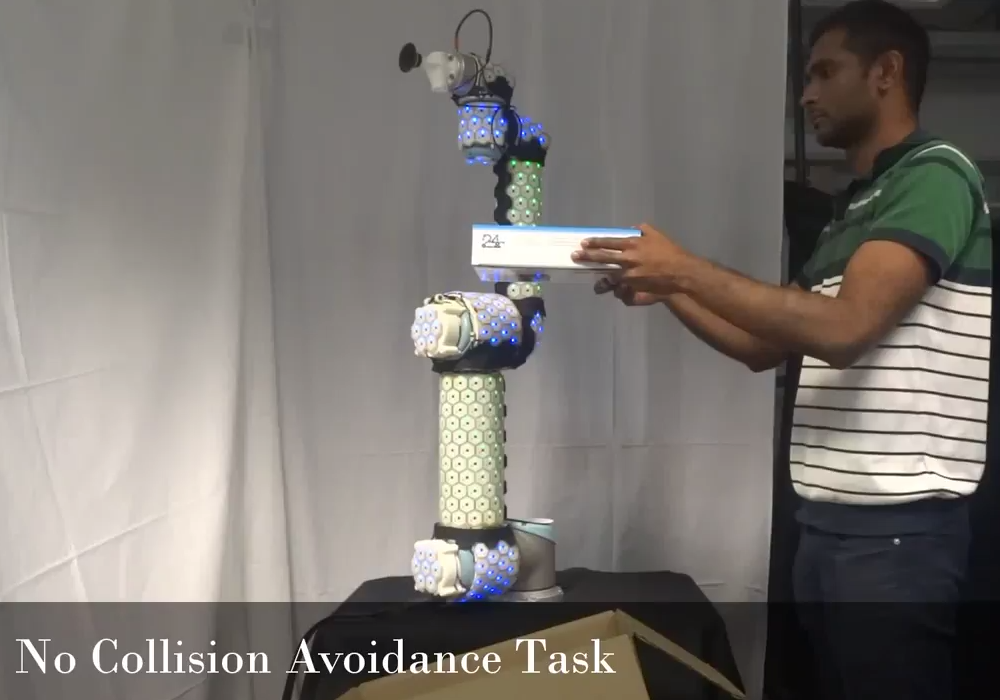
\includegraphics[width=6.5cm,height=6cm]{chapters/doa/images/delft/test_home2pick/cropped/test0_0-cropped.png}}
\end{subfigure}
\begin{subfigure}
[Colliding with Obstacle]{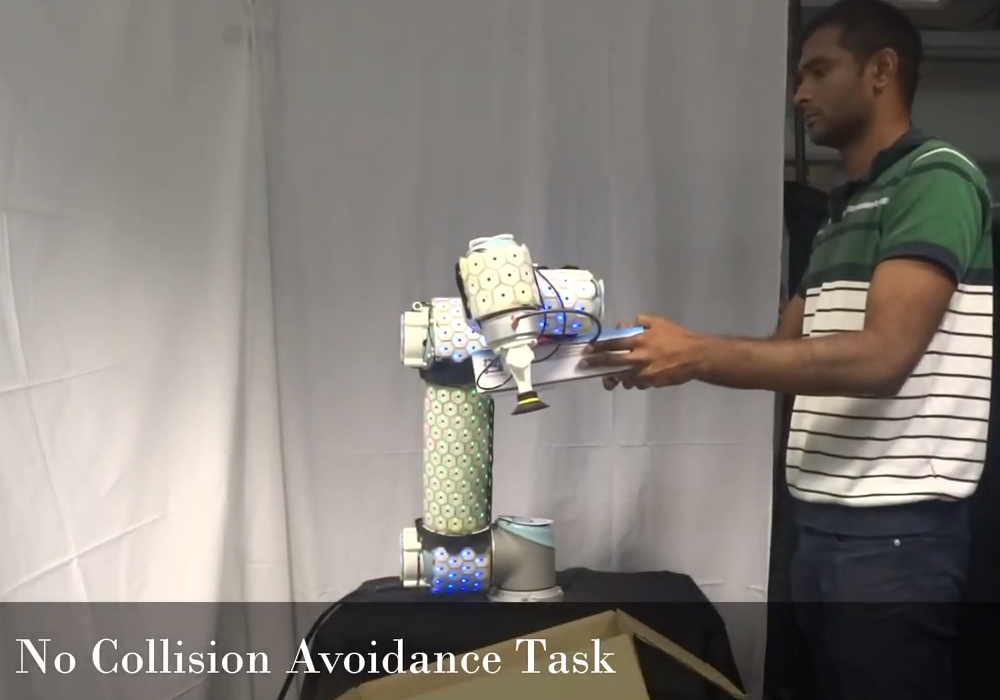
\includegraphics[width=6.5cm,height=6cm]{chapters/doa/images/delft/test_home2pick/cropped/test0_1-cropped.png}}
\end{subfigure}
\begin{subfigure}
[Avoiding Local Collisions]{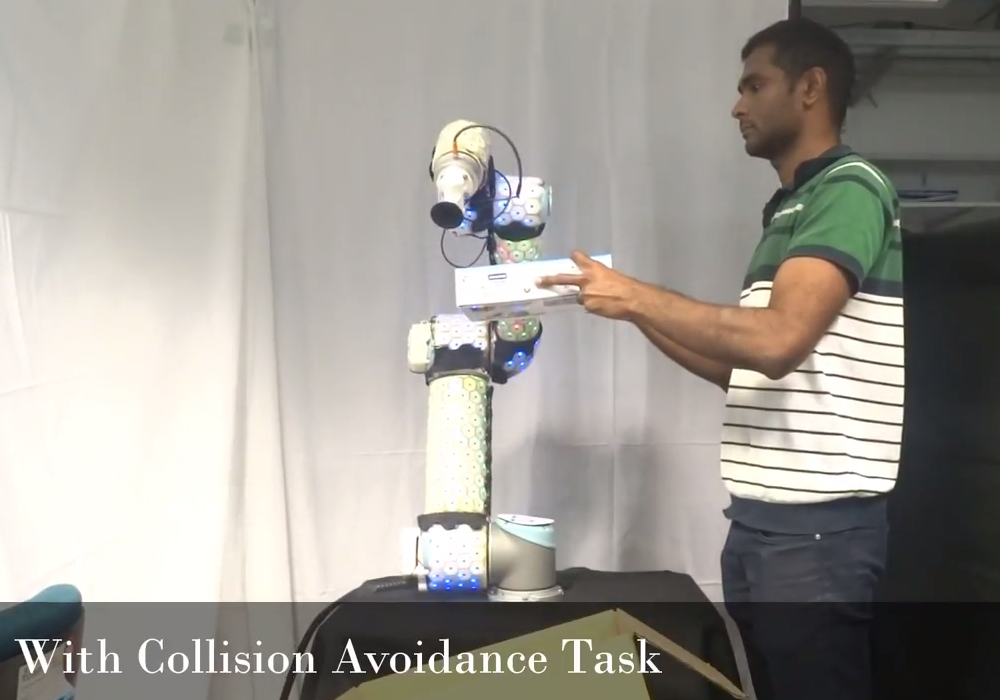
\includegraphics[width=6.5cm,height=6cm]{chapters/doa/images/delft/test_home2pick/cropped/test0_2-cropped.png}}
\end{subfigure}
\begin{subfigure}
[Place Position after avoiding Collisions]{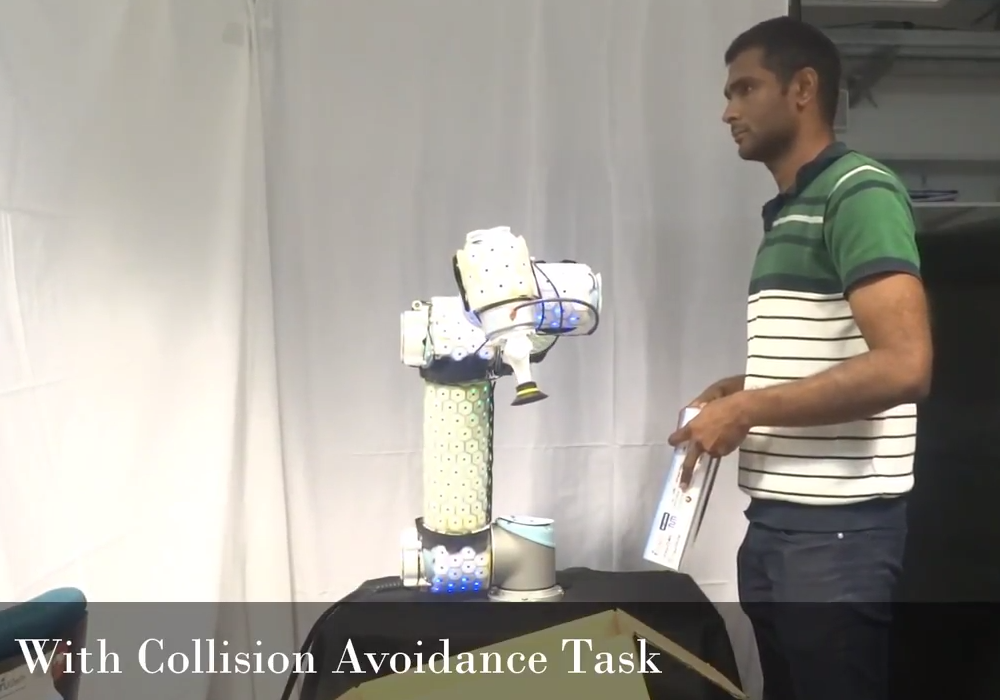
\includegraphics[width=6.5cm,height=6cm]{chapters/doa/images/delft/test_home2pick/cropped/test0_3-cropped.png}}
\end{subfigure}
\caption{Test 1: Trajectory execution from home to pick location with and without collision avoidance task in the controller stack. (b) shows the collision with the obstacle without the ability to avoid collision. (b) shows the collision avoidance of the arm though it gets stuck in the local minima but reaches the goal after the obstacle is removed.}
\label{fig:h2ptest1}
\end{figure}
The experimental validation done on the robot can be seen in these videos demonstrating three scenarios : \href{https://goo.gl/LVbQZz}{\textcolor{blue}{home to pick}}, \href{https://goo.gl/7jCqzA}{\textcolor{blue}{pick to place}}, \href{https://goo.gl/GP8KAA}{\textcolor{blue}{place to home}}. As it can be seen, a box is used as an obstacle to interrupt the executed path. Three tests are conducted at different obstacle locations introducing variability in the environment with these obstacles. Though there are many tests conducted, let us focus on certain tests and the behavior to illustrate the performance of the controller. The figure \ref{fig:h2ptest1} shows the test executing a trajectory from home to pick location with a fixed obstacle location as shown. (a) shows the initial state of the robot which is the home position and (b) shows the trajectory execution without any collision avoidance task to differentiate with the behavior generated by the controller with collision avoidance task. The robot evading collisions and its inability to reach the goal because of the object can be seen in (c) and (d). It gets stuck in local minima but manages to reach the goal after the object is removed. 

\begin{figure}[H]
\centering
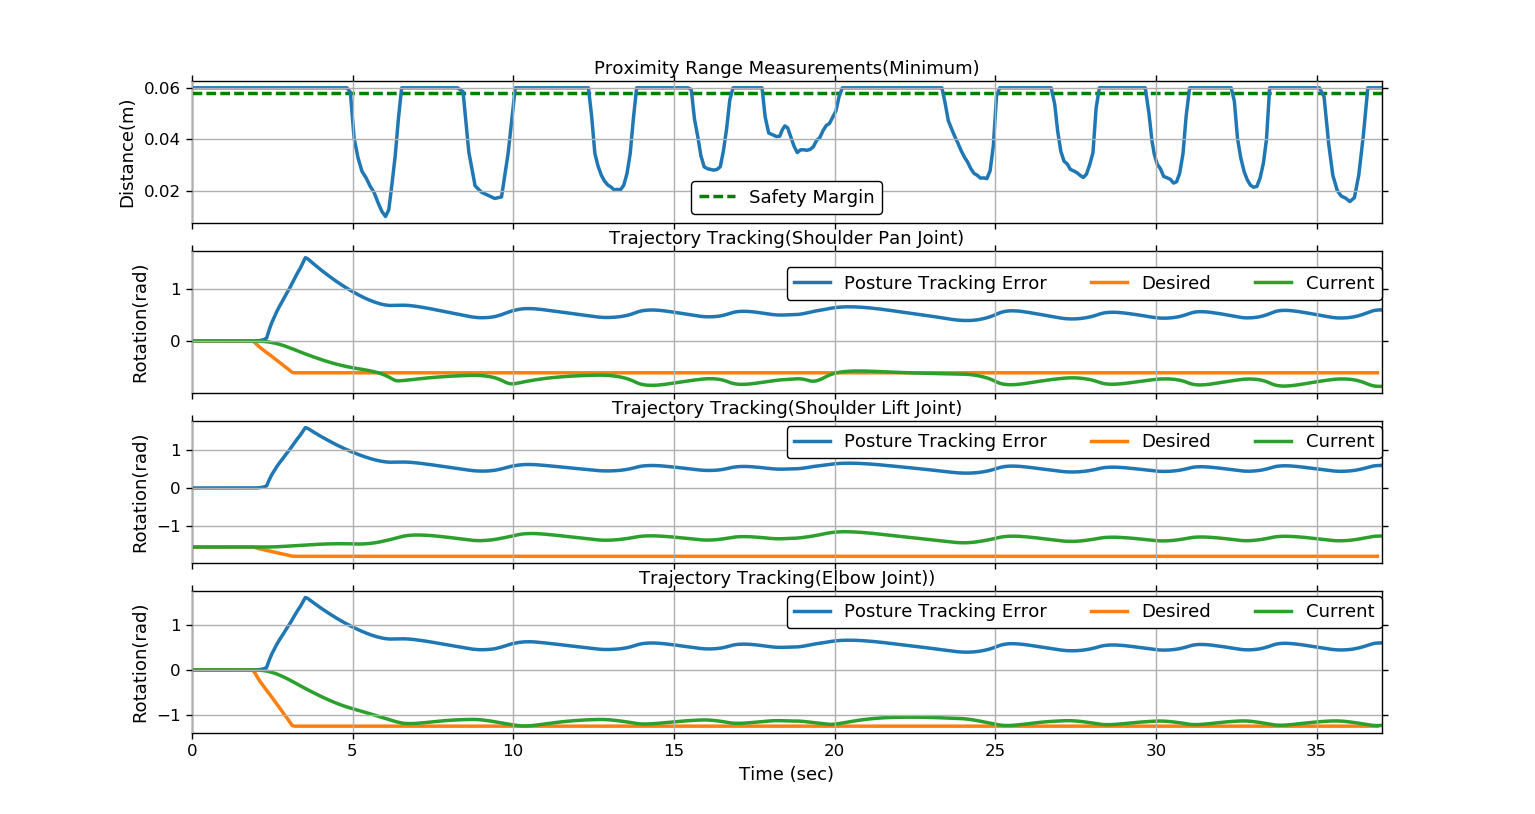
\includegraphics[width=18cm,height=13cm,center]{chapters/doa/images/delft/test_home2pick/plot_0.png}
\caption{Test 1: Plot during a Home to Pick Trajectory Execution: (1) shows the the min of range measurements from 8 skin sensor cells showing the vicinity of obstacles to the upper arm. (2),(3) and (4) shows the disturbances in the trajectory tracking when an obstacle is in the vicinity. The Posture tracking error doesn't settle to zero because of the local minima it encounters, resulting in continuous oscillations trying to go across the obstacle with a hope the obstacle will move away'}
\label{Home2Pick:test1}
\end{figure}
The plot in \ref{Home2Pick:test1}, \ref{Home2Pick:test2} shows the evolution of the trajectory tracking error and the proximity range measurements during the execution of a trajectory from home to pick with two obstacle locations respectively. The minimum of the proximity measurements of 8 cells is taken to show in the plots showing the presence of the obstacle close to the arm. The trajectory tracking error is the 2-norm of the current state of the robot and the posture command of the trajectory sequencer fed to posture task stacked in the solver.  Along with the trajectory error, the three major joints: shoulder pan, shoulder lift and the elbow joint states are plotted with the desired state to show the perturbations in response to the obstacle close to the arm. In both the plots, it can be observed that the trajectory tracking error increases rapidly irrespective of the obstacles at a proximity distance above the safety margin. This is because of the formulation as shown in \ref{eq:dd_ineq}, the collision avoidance task constrains the velocity of the skin cell based on the difference between the safety margin and the measured range. From the plots it can be observed, the difference is around 2 millimeter when there is no object close to the arm. The skin sensor range information is saturated to 6cm as the measurements above 6cm are highly nonlinear and unreliable. The 2mm difference along with smaller task gains reduces the speed of the robot. Though the saturation value can be adjusted to improve the speed of the robot behavior, the plots correspond to a non-ideal setting but still shows a robust collision avoidance. 


\begin{figure}[H]
\centering
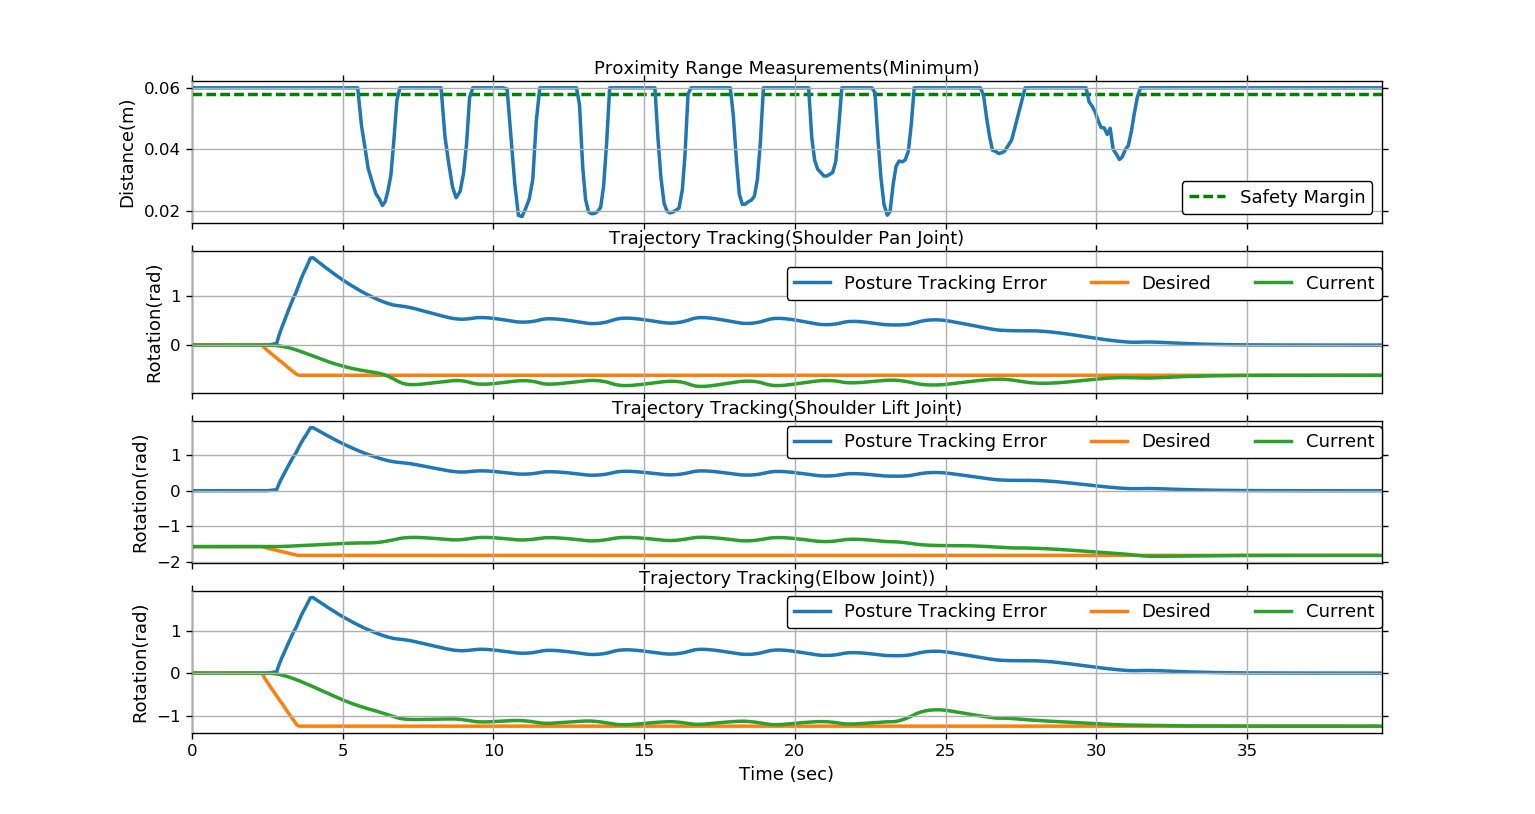
\includegraphics[width=18cm,height=13cm,center]{chapters/doa/images/delft/test_home2pick/plot_1.png}
\caption{Test 2: Plot during a Home to Pick Trajectory Execution: (1) shows the the min of range measurements from 8 skin sensor cells showing the vicinity of obstacles to the upper arm. (2),(3) and (4) shows the disturbances in the trajectory tracking when an obstacle is in the vicinity. The Posture tracking error settles to zero because the resulting deformation in trajectory was sufficient to evade obstacles and still achieve the goal.}
\label{Home2Pick:test2}
\end{figure}

In both the plots \ref{Home2Pick:test1} and \ref{Home2Pick:test2} , the disturbances in trajectory tracking when an obstacle is in the vicinity. In \ref{Home2Pick:test1}, the posture tracking error doesn’t settle to zero because of the local minima it encounters, resulting in continuous oscillations trying to go across the obstacle with a hope the obstacle will move away. In \ref{Home2Pick:test1}, the posture tracking error settles to zero because the resulting deformation in trajectory was sufficient to evade obstacles and still achieve the goal. In contrast to the previous plots, the plot \ref{Home2Pick:nocollision} shows the trajectory execution without collision avoidance task in the stack. As it can be seen in the video and in the plot, the trajectory execution was not affected while the arm literally goes across the obstacles which can be seen in the closeness of arm with the obstacles. The shoulder pan \& lift joint, elbow joint trajectory tracking is smooth without any disturbances like we saw in the previous plots validating the controller(with collision avoidance task) of taking actions in response to the obstacles in the vicinity.

\begin{figure}[H]
\centering
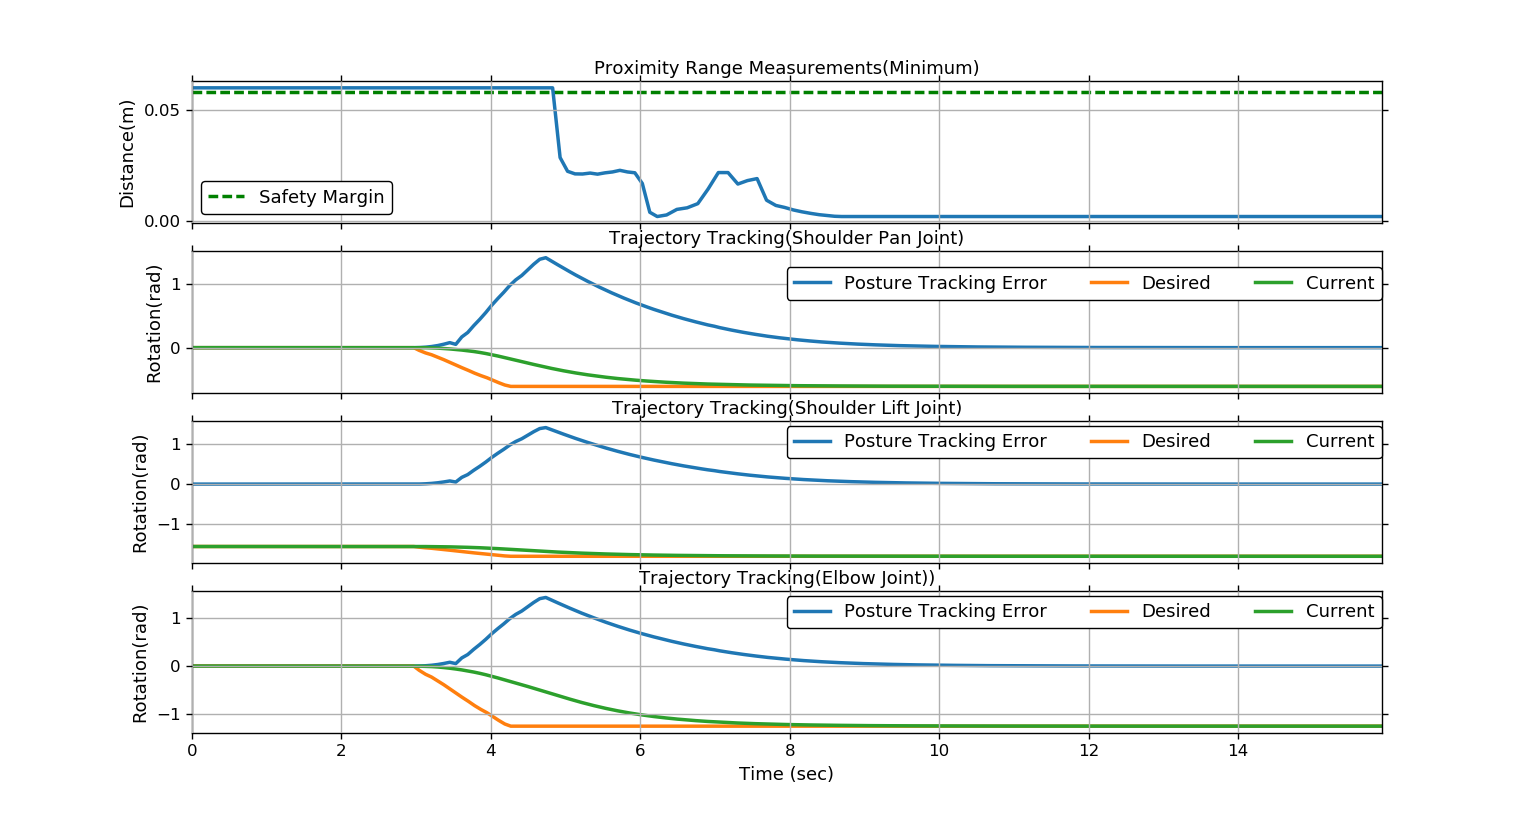
\includegraphics[width=18cm,height=13cm,center]{chapters/doa/images/delft/test_home2pick/plot_0_nocollision.png}
\caption{Test 1: Plot during a Home to Pick Trajectory Execution with no Collision Avoidance task in the Stack: (1) shows the the min of range measurements from 8 skin sensor cells showing the vicinity of obstacles to the upper arm. The sensor range drops close to zero showing the obstacle literally touching the robot. (2),(3) and (4) shows no disturbances in the trajectory tracking when an obstacle is in the vicinity. The Posture tracking error settles to zero after reaching the goal just by hitting the obstacle obviously because of no awareness.}
\label{Home2Pick:nocollision}
\end{figure}

The figure \ref{fig:p2ptest3} shows the test executing a trajectory from pick to place location with a fixed obstacle location as shown. (a) shows the initial state of the robot which is the pick position and (b) shows the trajectory execution without any collision avoidance task to differentiate with the behavior generated by the controller with collision avoidance task. The robot evading collisions and its ability to reach the goal by deforming the trajectory as seen in (c),(d) and (e) to reach (f). Similar natural behaviors can be seen in the rest of the videos referred previously.

\begin{figure}[H]
\centering
\begin{subfigure}
[Initial State - Pick Position]{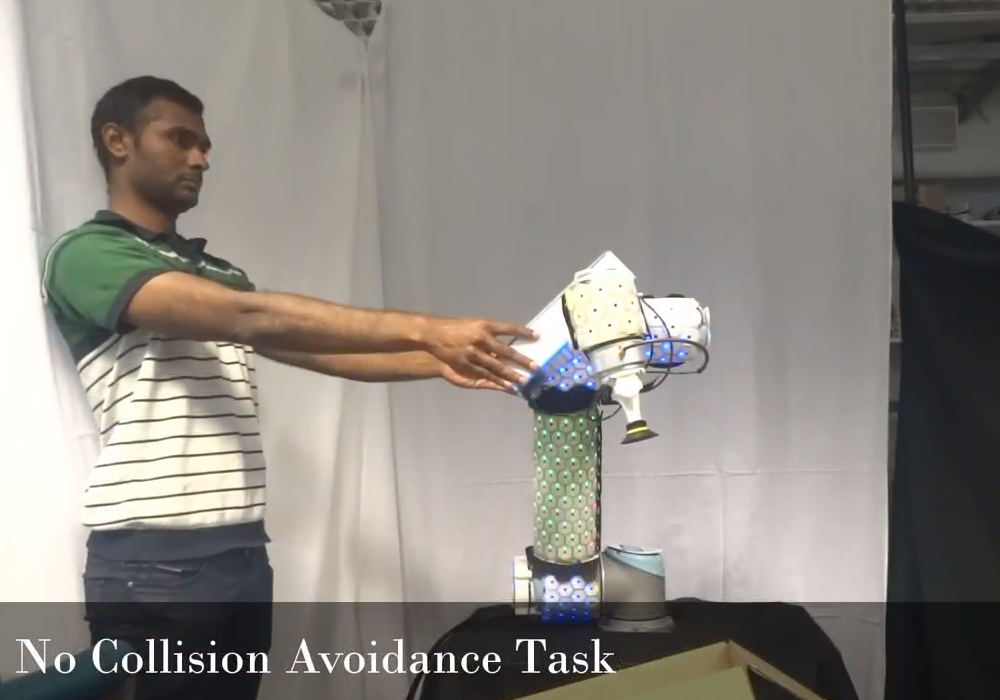
\includegraphics[width=6.5cm,height=6cm]{chapters/doa/images/delft/test_pick2place/cropped/test2_0-cropped.png}}
\end{subfigure}
\begin{subfigure}
[Colliding with Obstacle]{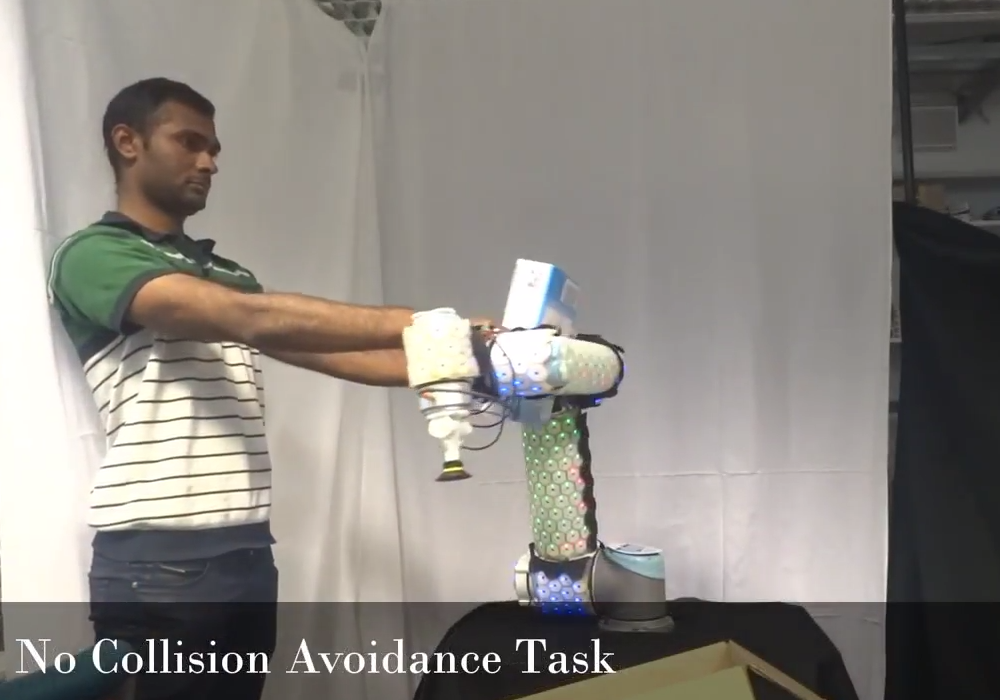
\includegraphics[width=6.5cm,height=6cm]{chapters/doa/images/delft/test_pick2place/cropped/test2_1-cropped.png}}
\end{subfigure}
\begin{subfigure}
[Avoiding Local Collisions 1/3]{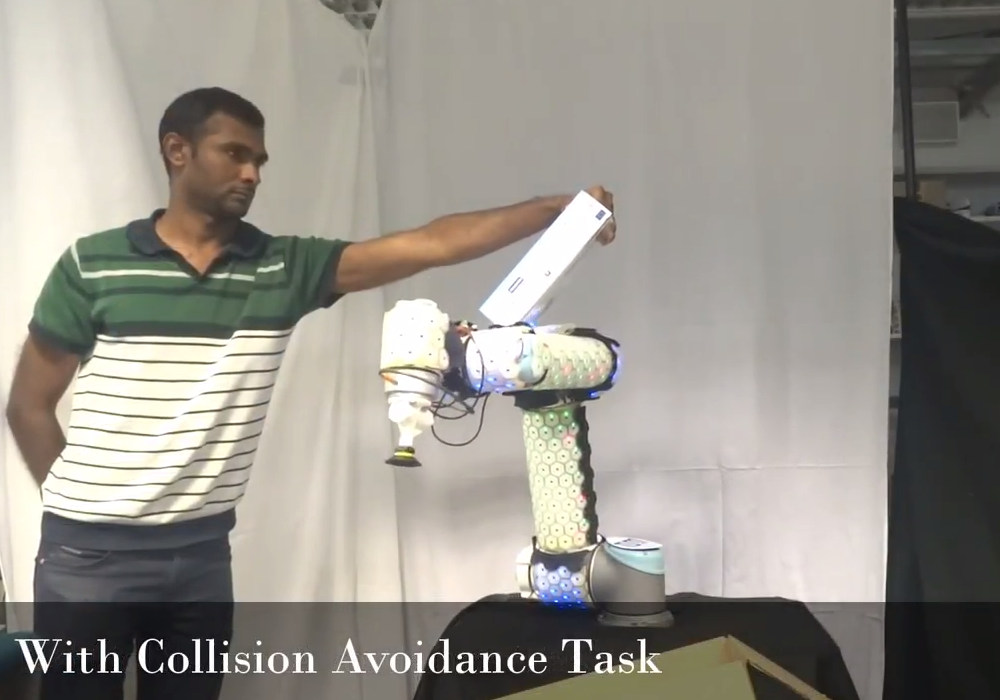
\includegraphics[width=6.5cm,height=6cm]{chapters/doa/images/delft/test_pick2place/cropped/test2_2-cropped.png}}
\end{subfigure}
\begin{subfigure}
[Avoiding Local Collisions 2/3]{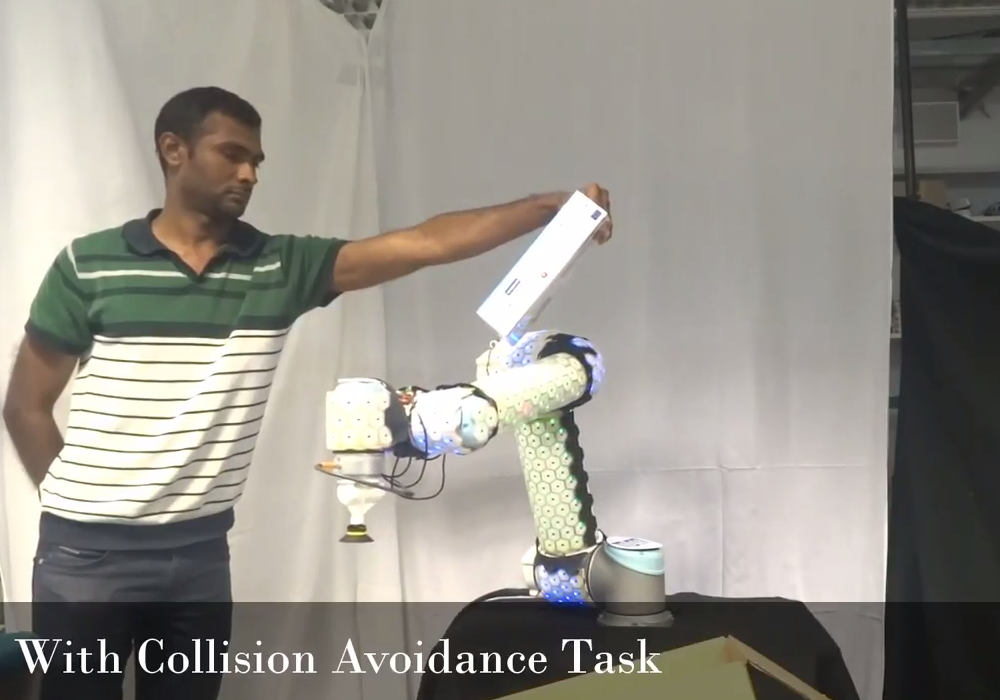
\includegraphics[width=6.5cm,height=6cm]{chapters/doa/images/delft/test_pick2place/cropped/test2_2_1-cropped.png}}
\end{subfigure}
\begin{subfigure}
[Avoiding Local Collisions 3/3]{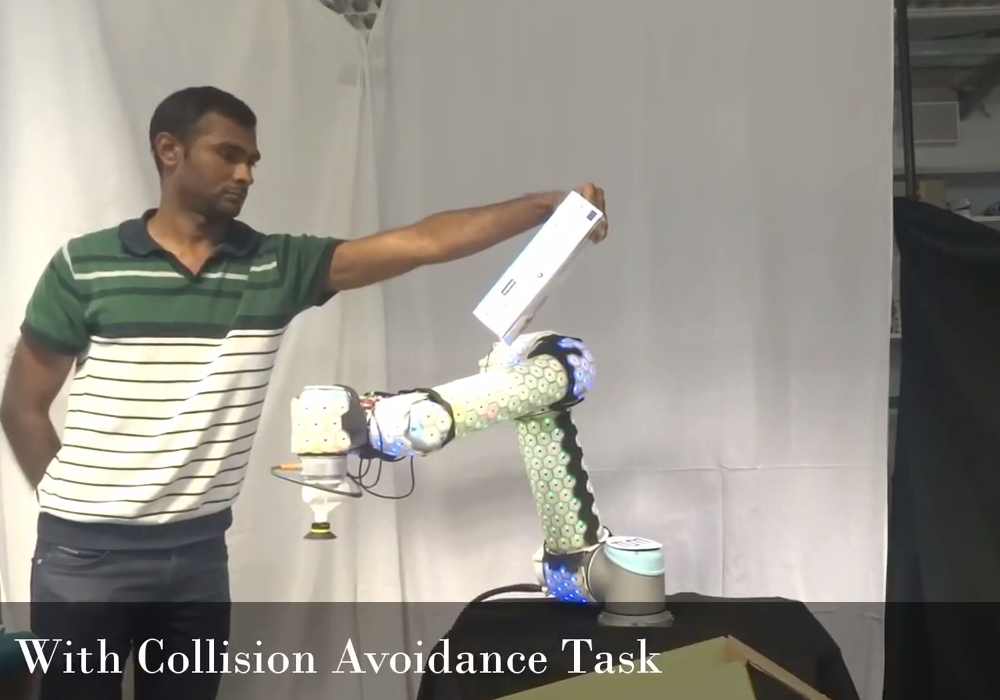
\includegraphics[width=6.5cm,height=6cm]{chapters/doa/images/delft/test_pick2place/cropped/test2_2_2-cropped.png}}
\end{subfigure}
\begin{subfigure}
[Final State - Place Position]{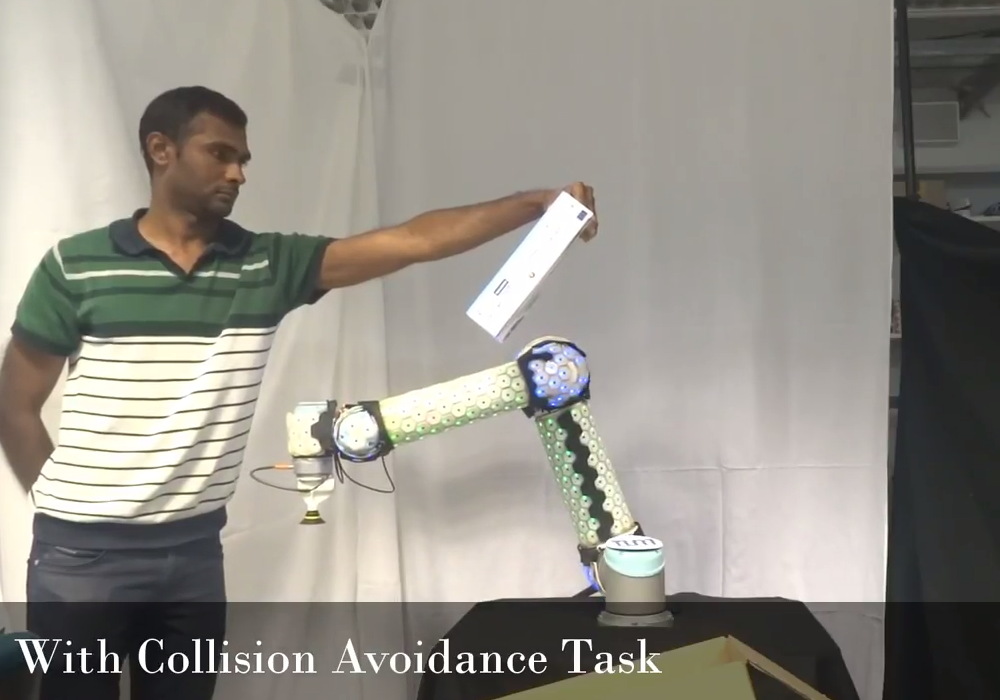
\includegraphics[width=6.5cm,height=6cm]{chapters/doa/images/delft/test_pick2place/cropped/test2_3-cropped.png}}
\end{subfigure}
\caption{Trajectory execution from pick to place location with and without collision avoidance task in the controller stack. (b) shows the collision with the obstacle without the ability to avoid collision. (b) shows the collision avoidance of the arm with a deformation in trajectory that allows the reach the goal with ease.}
\label{fig:p2ptest3}
\end{figure}

The reactive collision avoidance component after proper tuning is applied on a complete manipulation scenario involving multiple sequences of pick and place operations of boxes and shaving cans using a suction gripper in the end effector. The robot controller still holds the same ring of collision constraints in the upper arm for simplicity. The demonstration video is shown in this link \href{https://goo.gl/PLbKdb}{\textcolor{blue}{here}} with snapshots shown in . 

\begin{figure}[H]
\centering
\begin{subfigure}
[Grasping with a suction gripper]{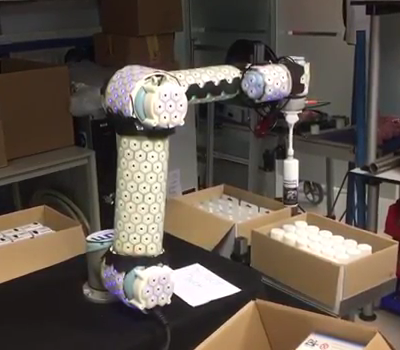
\includegraphics[width=6.5cm,height=6cm]{chapters/doa/images/delft/complete/suckstill-cropped.png}}
\end{subfigure}
\begin{subfigure}
[Avoiding Obstacles]{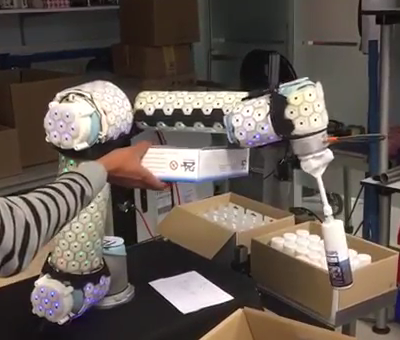
\includegraphics[width=6.5cm,height=6cm]{chapters/doa/images/delft/complete/avoiding-cropped.png}}
\end{subfigure}
\caption{Illustrating obstacle avoidance while picking and placing small objects using a suction gripper. The full scenario video can be seen in this \href{https://goo.gl/PLbKdb}{\textcolor{blue}{video}}.}
\label{fig:final_scenario}
\end{figure}

\begin{figure}[H]
\centering
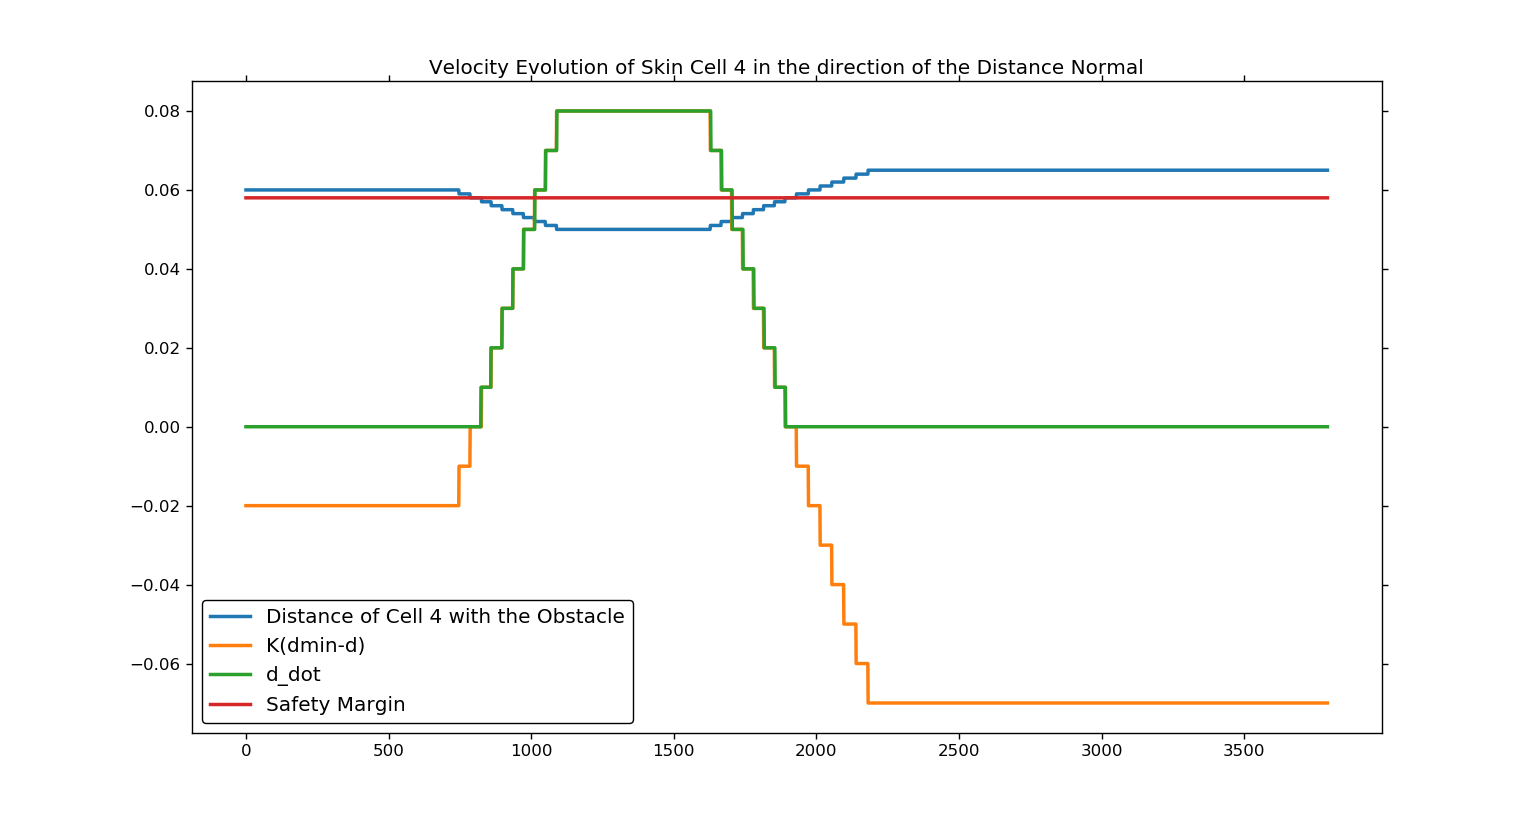
\includegraphics[width=18cm,height=8cm,center]{chapters/doa/images/delft/plot_satisfy.png}
\caption{Plot showing the evolution of a skin cell velocity satisfying the \ref{eq:dd_ineq} when the other cells have no obstacles in the vicinity.}
\label{fig:plotsatisfy}
\end{figure}

Another interesting aspect of the controller is the ability to compromise with the collision constraint inequalities in case the modeled constraint is not feasible without breaking the solver making the controller reliable. The plot \ref{fig:plotsatisfy} shows the change in velocity of a specific skin cell in response to changing obstacle in the vicinity. This plot is generated by simulating a distance signal to cell number 4 (among the 8 cells) around the safety margin while keeping the other skin cell values equal to 0.6 which is 10 times far away from the safety margin. This shows a practical feasibility of the goal thus resulting in a behavior inline with the formulated collision avoidance constraint in \ref{eq:dd_ineq}. 

But when we have a situation where the obstacles are around the arm in all directions within or beyond the safety margin, the controller compromises with the collision avoidance constraint as shown in the plot. This might look like a design issue but this is purely because of the nature of the HQP solver which compromises with the goal to achieve the maximum possible without breaking the controller or generating bad motion behaviors making it reliable. 

\begin{figure}[H]
\centering
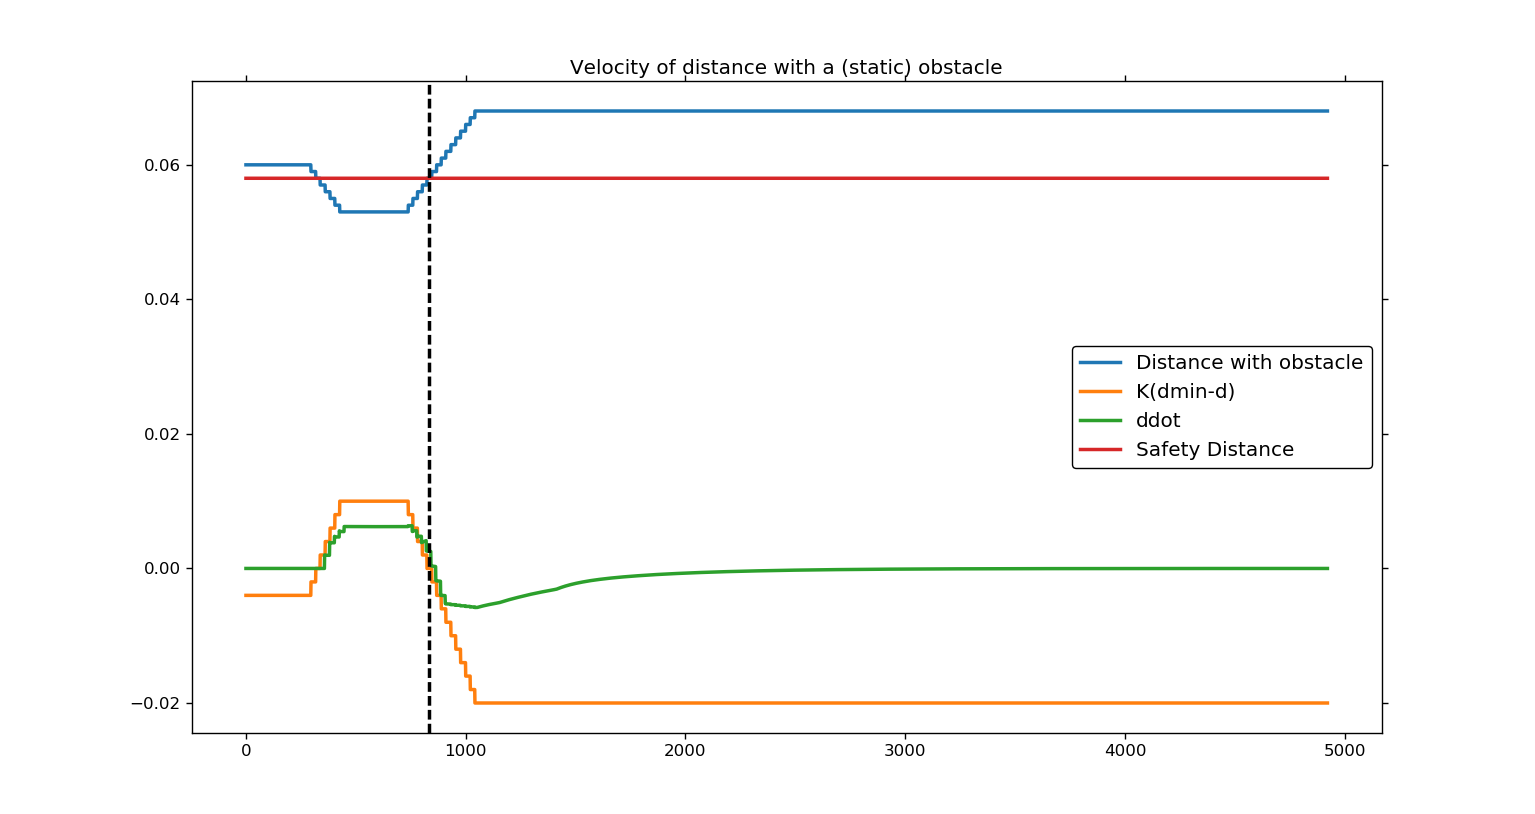
\includegraphics[width=18cm,height=8cm,center]{chapters/doa/images/delft/plot_unsatisfy.png}
\caption{Plot showing the evolution of a skin cell velocity not satisfying the \ref{eq:dd_ineq} when the other cells have obstacles in the vicinity but not inside the safety margin. The other skin cells are simulated to measure 6cm which is just 2mm from the safety margin. This constrains the upper arm in achieving a skin cell velocity satisfying the \ref{eq:dd_ineq} as the control believes there is an obstacle still around hence resulting in safer motions.}
\label{fig:plot_unsatisfy}
\end{figure}







\section{Conclusion{\color{red}(to be updated)}}
\label{doa:conclusion}
This chapter presented the technologies that have been developed in the FiaD project to augment collaborative robot manipulators with dynamic obstacle avoidance. All these technologies: a proximity-sensing robot skin, a reactive path planning solution and a robot motion control strategy, have been validated in laboratory prototypes. Also, a preliminary prototype of an integrated solution based on these technologies has been tested in simulation. Effort on making the collision avoidance component generic enough to handle all the skin sensors by feeding only the minimal activated skin cells.  

\ifdefined\included
\else
\bibliographystyle{acm}
\bibliography{These}
\end{document}
\fi